%%%%%%%%%%%%%%%%%%%%%%%%%%%%%%%%%%%%%%%%%%%%%%%%%%%%%%%%%%%%%%%%%%%%%%%%%%%%%%%%
%% Plantilla de memoria en LaTeX para la ETSIT - Universidad Rey Juan Carlos
%%
%% Por Gregorio Robles <grex arroba gsyc.urjc.es>
%%     Grupo de Sistemas y Comunicaciones
%%     Escuela Técnica Superior de Ingenieros de Telecomunicación
%%     Universidad Rey Juan Carlos
%% (muchas ideas tomadas de Internet, colegas del GSyC, antiguos alumnos...
%%  etc. Muchas gracias a todos)
%%
%% La última versión de esta plantilla está siempre disponible en:
%%     https://github.com/gregoriorobles/plantilla-memoria
%%
%% Para obtener PDF, ejecuta en la shell:
%%   make
%% (las imágenes deben ir en PNG o JPG)

%%%%%%%%%%%%%%%%%%%%%%%%%%%%%%%%%%%%%%%%%%%%%%%%%%%%%%%%%%%%%%%%%%%%%%%%%%%%%%%%

\documentclass[a4paper, 12pt]{book}
%\usepackage[T1]{fontenc}

\usepackage[a4paper, left=2.5cm, right=2.5cm, top=3cm, bottom=3cm]{geometry}
\usepackage{times}
\usepackage[utf8]{inputenc}
\usepackage[spanish]{babel} % Comenta esta línea si tu memoria es en inglés
\usepackage{url}
%\usepackage[dvipdfm]{graphicx}
\usepackage{graphicx}
\usepackage{float}  %% H para posicionar figuras
\usepackage[nottoc, notlot, notlof, notindex]{tocbibind} %% Opciones de índice
\usepackage{latexsym}  %% Logo LaTeX

\title{Memoria del Proyecto}
\author{Nombre del autor}

\renewcommand{\baselinestretch}{1.5}  %% Interlineado

\begin{document}

\renewcommand{\refname}{Bibliografía}  %% Renombrando
\renewcommand{\appendixname}{Apéndice}

%%%%%%%%%%%%%%%%%%%%%%%%%%%%%%%%%%%%%%%%%%%%%%%%%%%%%%%%%%%%%%%%%%%%%%%%%%%%%%%%
% PORTADA

\begin{titlepage}
\begin{center}
\includegraphics[scale=0.8]{img/URJ_logo_Color_POS.png}

\vspace{1.75cm}

\Large
2039 - GRADO EN INGENIERÍA EN SISTEMAS AUDIOVISUALES Y MULTIMEDIA (FUENLABRADA)

\vspace{0.4cm}

\large
Curso Académico 2021/2022

\vspace{0.8cm}

Trabajo Fin de Grado

\vspace{2.5cm}

\LARGE
IMPLEMENTACIÓN DE FUNCIONALIDADES EN LEARNINGML: RECONOCIMIENTO DE AUDIO

\vspace{4cm}

\large
Autor : Álvaro del Hoyo Arias \\
Tutor : Dr. Gregorio Robles Martínez \\
Co-Tutor : Juan David Rodríguez García
\end{center}
\end{titlepage}

\newpage
\mbox{}
\thispagestyle{empty} % para que no se numere esta pagina


%%%%%%%%%%%%%%%%%%%%%%%%%%%%%%%%%%%%%%%%%%%%%%%%%%%%%%%%%%%%%%%%%%%%%%%%%%%%%%%%
%%%% Para firmar
\clearpage
\pagenumbering{gobble}
\chapter*{}

\vspace{-4cm}
\begin{center}
\LARGE
\textbf{Trabajo Fin de Grado}

\vspace{1cm}
\large
Implementación de Funcionalidades en LearningML: \\ Reconocimiento de Audio

\vspace{1cm}
\large
\textbf{Autor :} Álvaro del Hoyo Arias \\
\textbf{Tutor :} Dr. Gregorio Robles Martínez \\
\textbf{Co-Tutor :} Juan David Rodríguez García

\end{center}

\vspace{1cm}
La defensa del presente Proyecto Fin de Carrera se realizó el día \qquad$\;\,$ de \qquad\qquad\qquad\qquad \newline de 2021, siendo calificada por el siguiente tribunal:


\vspace{0.5cm}
\textbf{Presidente:}

\vspace{1.2cm}
\textbf{Secretario:}

\vspace{1.2cm}
\textbf{Vocal:}


\vspace{1.2cm}
y habiendo obtenido la siguiente calificación:

\vspace{1cm}
\textbf{Calificación:}


\vspace{1cm}
\begin{flushright}
Fuenlabrada, a \qquad$\;\,$ de \qquad\qquad\qquad\qquad de 2021
\end{flushright}

%%%%%%%%%%%%%%%%%%%%%%%%%%%%%%%%%%%%%%%%%%%%%%%%%%%%%%%%%%%%%%%%%%%%%%%%%%%%%%%%
%%%% Dedicatoria

\chapter*{}
\pagenumbering{Roman} % para comenzar la numeracion de paginas en numeros romanos
\begin{flushright}
\textit{Dedicado\\
	al Atleti,\\que me hizo no dejar de creer\\nunca\\
	mi familia,\\que siempre me levantó\\cuando me caía,\\
	mis amigos,\\que han estado a mi lado\\en este maratón que es la vida.}
\end{flushright}

%%%%%%%%%%%%%%%%%%%%%%%%%%%%%%%%%%%%%%%%%%%%%%%%%%%%%%%%%%%%%%%%%%%%%%%%%%%%%%%%
%%%% Agradecimientos

\chapter*{Agradecimientos}
%\addcontentsline{toc}{chapter}{Agradecimientos} % si queremos que aparezca en el índice
\markboth{AGRADECIMIENTOS}{AGRADECIMIENTOS} % encabezado 

Siempre hay que empezar por el principio, y el principio de todo fue cosa de mis padres, que me han dado todo lo que han podido, que me han apoyado en todas mis decisiones, que nunca han dejado de creer en mi y que siempre han buscado una forma de hacerme feliz.

También hay que mencionar a mi hermana, que me ayuda, me apoya, me hace sonreír y siempre está a mi lado cuando la necesito.

No me voy a olvidar de vosotros, de los que quedábamos por las mañanas en la cafetería, para un café, lo que surja, y subir a clase, son muchos años estando juntos, hemos pasado de no ser nada, desconocidos, a ser más que amigos, hermanos.

Gracias a todos, a los que siguieron hasta el final, a los que se quedaron por el camino.

Gracias.

%%%%%%%%%%%%%%%%%%%%%%%%%%%%%%%%%%%%%%%%%%%%%%%%%%%%%%%%%%%%%%%%%%%%%%%%%%%%%%%%
%%%% Resumen

\chapter*{Resumen}
%\addcontentsline{toc}{chapter}{Resumen} % si queremos que aparezca en el índice
\markboth{RESUMEN}{RESUMEN} % encabezado

Este proyecto consiste en añadir funcionalidad de reconocimiento de audio a la aplicación web \texttt{LearningML}\footnote{\url{https://learningml.org/editor/}}. \texttt{LearningML} nació con la intención de ayudar a los profesores de secundaria en explicar de una manera más simple el funcionamiento de las técnicas de \texttt{Machine Learning} y las posibilidades que esto ofrece a alumnos de entre 12 y 16 años.

El proyecto se ha implementado en Angular, que es un entorno de trabajo que utiliza HTML y CSS para construir aplicaciones web, además de utilizar TypeScript por debajo para realizar toda funcionalidad dentro de la propia aplicación.

Este proyecto se ha realizado teniendo en cuenta que debía de tener una interfaz sencilla y amigable, en la que la obtención de datos fuera simple, pero efectiva.

%%%%%%%%%%%%%%%%%%%%%%%%%%%%%%%%%%%%%%%%%%%%%%%%%%%%%%%%%%%%%%%%%%%%%%%%%%%%%%%%
%%%% Resumen en inglés

\chapter*{Summary}
%\addcontentsline{toc}{chapter}{Summary} % si queremos que aparezca en el índice
\markboth{SUMMARY}{SUMMARY} % encabezado

This project consists of adding functionality for audio recognition to the web app \texttt{LearningML}\footnote{\url{https://learningml.org/editor/}}. \texttt{LearningML} was born with the intention of helping teachers to explain in a simpler way the operation of the \texttt{Machine Learning} and the possibilities that this offers to students between 12 and 16 years old.

The project has been implemented with Angular, which is a work environment that uses HTML and CSS to build web applications, in addition to using TypeScript underneath to perform all functionality within the application itself.

This project has been carried out bearing in mind that it should have a simple and friendly interface, in which data collection was simple, but effective.


%%%%%%%%%%%%%%%%%%%%%%%%%%%%%%%%%%%%%%%%%%%%%%%%%%%%%%%%%%%%%%%%%%%%%%%%%%%%%%%%
%%%%%%%%%%%%%%%%%%%%%%%%%%%%%%%%%%%%%%%%%%%%%%%%%%%%%%%%%%%%%%%%%%%%%%%%%%%%%%%%
% ÍNDICES %
%%%%%%%%%%%%%%%%%%%%%%%%%%%%%%%%%%%%%%%%%%%%%%%%%%%%%%%%%%%%%%%%%%%%%%%%%%%%%%%%

% Las buenas noticias es que los índices se generan automáticamente.
% Lo único que tienes que hacer es elegir cuáles quieren que se generen,
% y comentar/descomentar esa instrucción de LaTeX.

%%%% Índice de contenidos
\tableofcontents 
%%%% Índice de figuras
\cleardoublepage
%\addcontentsline{toc}{chapter}{Lista de figuras} % para que aparezca en el indice de contenidos
\listoffigures % indice de figuras
%%%% Índice de tablas
%\cleardoublepage
%\addcontentsline{toc}{chapter}{Lista de tablas} % para que aparezca en el indice de contenidos
%\listoftables % indice de tablas


%%%%%%%%%%%%%%%%%%%%%%%%%%%%%%%%%%%%%%%%%%%%%%%%%%%%%%%%%%%%%%%%%%%%%%%%%%%%%%%%
%%%%%%%%%%%%%%%%%%%%%%%%%%%%%%%%%%%%%%%%%%%%%%%%%%%%%%%%%%%%%%%%%%%%%%%%%%%%%%%%
% INTRODUCCIÓN %
%%%%%%%%%%%%%%%%%%%%%%%%%%%%%%%%%%%%%%%%%%%%%%%%%%%%%%%%%%%%%%%%%%%%%%%%%%%%%%%%

\cleardoublepage
\chapter{Introducción}
\label{chap:intro} % etiqueta para poder referenciar luego en el texto con \ref{chap:intro}
\pagenumbering{arabic} % para empezar la numeración de página con números

En nuestros días, es un hecho incuestionable la ingente cantidad de información que se genera cada segundo en nuestro planeta. También puede aportar enorme valor a cualquier entidad o puede suponer un consumo excesivo de recursos. El análisis inteligente de este tipo de información está empezando a ser un requisito para la supervivencia de muchas empresas y organizaciones~\cite{mate2014big}.

Las técnicas de \texttt{Machine Learning} son un subconjunto de la inteligencia artificial~~\cite{zhang2020machine} que permite analizar una cantidad de datos muy grande de una manera eficiente y buena. La necesidad de que apareciese algo que fuera capaz de analizar, ordenar, definir y predecir futuros datos es algo que ha ido apareciendo con el paso de las décadas, sólo en 2018 se generaron 33 zettabytes de datos, que supone un incremento del 16,5\% respecto de los datos generados en 2009~\cite{cantidad-datos}. El problema a la hora de realizar un análisis de estos datos está en la complejidad de los mismos, que hace que un ser humano pueda tardar años en realizar un análisis al que una máquina bien preparada únicamente dedicaría segundos. Por ello es tan importante el desarrollo del \texttt{Machine Learning}, ya que permite procesar grandes cantidades de datos complejos, transformándolos en información más sencilla y legible para nosotros, los seres humanos.

Partiendo de esta rama, el análisis de audio no se ha quedado atrás y se ha convertido en algo normal en nuestro día a día, aplicaciones como \texttt{Alexa} o \texttt{Siri}, de \texttt{Amazon} y \texttt{Apple} respectivamente, hacen que el reconocimiento de patrones audibles parezca algo sencilla, no obstante, estas aplicaciones llevan miles de horas de trabajo detrás.

\section{Presentación de la aplicación}
\label{sec:presentacion}

\texttt{LearningML} es una aplicación creada por Juan David Rodríguez que permite llevar el \texttt{Machine Learning} a un entorno más amigable, haciendo que el reconocimiento fácil o el reconocimiento de patrones en textos se pueda hacer, observar y comprobar de una manera sencilla y eficiente~\cite{garcia2020learningml}. Hace uso de redes neuronales, aunque también dispone de otros algoritmos como pueda ser KNN. Esto hace que sea una herramienta muy útil a nivel escolar, pero esa no es su única utilidad, ya que incluso la gente que entiende y comprende cómo funcionan los algoritmos antes mencionados pueden llevar a cabo pruebas bastante exhaustivas sobre la importancia de los parámetros que se vayan a utilizar~\cite{garcia2019developing}. También permite la descarga del modelo en un fichero en formato JSON, para así no tener que crear de nuevo el modelo si se quiere continuar haciendo pruebas. \texttt{LearningML} ha sido probado ya con éxito en entornos educativos formales para jóvenes de entre 12 y 16 años~\cite{rodriguez2021evaluation}.

Además de todas estas funcionalidades, tiene la posibilidad de registro, para mantener los modelos a salvo en la nube, e incluso da la posibilidad de exportar los proyectos a Scratch.

Este proyecto consiste en la integración de ubn nuevo tipo de análisis: el análisis de audio.

\section{Estructura de la memoria}
\label{sec:estructura}

\begin{itemize}
  \item \textbf{Capítulo \ref{chap:intro}: Introducción. } Se explica qué es, para qué se usa  y cuál es el objetivo de la página web \textit{LearningML}\footnote{\url{https://learningml.org/editor/}}.
  
  \item \textbf{Capítulo \ref{chap:objetivos}: Objetivos. } Se describen los objetivos, principales y específicos, del trabajo realizado.
  
  \item \textbf{Capítulo \ref{chap:estado}: Estado del arte. } Se hace una breve explicación sobre cada una de las tecnologías utilizadas en el proyecto.
  
  \item \textbf{Capítulo \ref{chap:diseño-implementacion}: Diseño e implementación. } Hay una descripción y explicación detallada sobre la estructura de LearningML, así como el desarrollo e implementación del análisis de audio.
  
  \item \textbf{Capítulo \ref{chap:experimentos-validacion}: Experimentos y validación. } Se prueba la funcionalidad implementada con varios ejemplos.
  
  \item \textbf{Capítulo \ref{chap:resultados}: Resultados. } Se muestran y comentan los resultados obtenidos en el apartado anterior.
  
  \item \textbf{Capítulo \ref{chap:conclusiones}: Conclusiones. } Se comprueba, repasa y explica la resolución del trabajo.
 
\end{itemize}

%%%%%%%%%%%%%%%%%%%%%%%%%%%%%%%%%%%%%%%%%%%%%%%%%%%%%%%%%%%%%%%%%%%%%%%%%%%%%%%%
%%%%%%%%%%%%%%%%%%%%%%%%%%%%%%%%%%%%%%%%%%%%%%%%%%%%%%%%%%%%%%%%%%%%%%%%%%%%%%%%
% OBJETIVOS %
%%%%%%%%%%%%%%%%%%%%%%%%%%%%%%%%%%%%%%%%%%%%%%%%%%%%%%%%%%%%%%%%%%%%%%%%%%%%%%%%

\cleardoublepage % empezamos en página impar
\chapter{Objetivos} % título del capítulo (se muestra)
\label{chap:objetivos} % identificador del capítulo (no se muestra, es para poder referenciarlo)

El objetivo de este proyecto consiste en implementar el reconocimiento de audio en la aplicación web \textit{LearningML}.

\section{Objetivo general} % título de sección (se muestra)
\label{sec:objetivo-general} % identificador de sección (no se muestra, es para poder referenciarla)

El principal objetivo que persigue el creador de la aplicación web, Juan David Rodríguez García, es ayudar a los jóvenes, entre 12 y 16 años, a entender en qué consisten las técnicas de \textit{Machine Learning}. Para ello implementó el reconocimiento de imágenes y textos mediante el uso de redes neuronales, después se añadieron nuevos algoritmos, como KNN o Naïve Bayes.

Mi objetivo en este proyecto consiste en implementar técnicas de reconocimiento de audio, siguiendo la dinámica de los otros algoritmos de reconocimiento (imágenes y texto) y tratando de hacerlo de la manera más sencilla e intuitiva posible para el usuario.

\section{Objetivos específicos}
\label{sec:objetivos-especificos}

\begin{itemize}

  \item Comprender cómo funciona el análisis de audio, para saber qué hay que obtener de cada muestra.
  \item Analizar la arquitectura de \textit{LearningML}, para que la implementación siga la línea de lo ya creado.
  \item Añadir en la interfaz un apartado para analizar audio.
  \item Crear un componente en \textit{Angular} que recoja los datos del usuario, por micrófono o mediante un fichero de audio.
  \item Analizar los datos obtenidos.

\end{itemize}


\section{Planificación temporal}
\label{sec:planificacion-temporal}

La idea de empezar a realizar este proyecto surgió por enero de 2021, pero no fue hasta mediados de febrero de ese mismo año que comencé a buscar qué podía hacer.

Tras contactar con el Dr. Gregorio Robles, quien me impartió la asignatura de \textit{Protocolos para la Transmisión de Audio y Vídeo}, me propuso realizar implementaciones para esta aplicación web. Había bastantes posibilidades que poder implementar, pero finalmente me decidí por el análisis de audio, ya que era algo que tenía más cercano por haber cursado una asignatura sobre este tema en años anteriores, \textit{Tratamiento Digital del Sonido}.

Una vez confirmé con Gregorio que me interesaba hacer esa implementación, me puso en contacto con el creador de la página, Juan David Rodríguez García, quien me explicó el objetivo que perseguía con este proyecto y qué pretendía conseguir con el análisis de audio.

Hubo dos semanas de comprensión de los lenguajes utilizados, \textit{Angular} y \textit{TypeScript}, así como de reuniones con Juan David para que nos explicara, tanto a mi como al resto de alumnos que desarrollaban más funcionalidades, cómo funcionaba la arquitectura de la página.

Una vez comprendí cómo funcionaba, comencé con la implementación. Primero tuve que crear los componentes que iba a utilizar, así como introducirlos en los otros componentes principales y dejarlos siguiendo una estructura similar a los componentes ya creados. Una vez ya estaba todo creado, comenzó la tarea complicada: rellenar las funciones y procedimientos de manera que fueran funcionales.

Después de unos meses de búsquedas y de desarrollos que no llegaban a ninguna solución, conseguí terminar la implementación de este analizador de audio.


%%%%%%%%%%%%%%%%%%%%%%%%%%%%%%%%%%%%%%%%%%%%%%%%%%%%%%%%%%%%%%%%%%%%%%%%%%%%%%%%
%%%%%%%%%%%%%%%%%%%%%%%%%%%%%%%%%%%%%%%%%%%%%%%%%%%%%%%%%%%%%%%%%%%%%%%%%%%%%%%%
% ESTADO DEL ARTE %
%%%%%%%%%%%%%%%%%%%%%%%%%%%%%%%%%%%%%%%%%%%%%%%%%%%%%%%%%%%%%%%%%%%%%%%%%%%%%%%%

\cleardoublepage
\chapter{Estado del arte}
\label{chap:estado}

\section{Inteligencia Artificial}
\label{sec:ia}

La \texttt{Inteligencia Artificial} es la habilidad de los ordenadores para hacer actividades que normalmente requieren inteligencia humana~\cite{rouhiainen2018inteligencia}. No obstante, también podría definirse como la capacidad de analizar mediante el uso de algoritmos, aprender de los datos analizados y utilizar lo aprendido tomando decisiones similares a las que tomaría un ser humano en su lugar.

El impacto que la \texttt{Inteligencia Artificial} puede tener en nuestras vidas no se limitará solo al ámbito científico, ya que bien utilizada, podría utilizarse para sustituir a los seres humanos en tareas que puedan resultar peligrosas. Además, en el ámbito empresarial, se podría obtener bastante ventaja competitiva si se pudiera ``predecir'' el futuro de una manera más o menos acertada.

\section{Machine Learning}
\label{sec:machine-learning}

El \texttt{Machine Learning}~\cite{rouhiainen2018inteligencia}, o Aprendizaje Máquina, es uno de los principales enfoques utilizados en la inteligencia artificial moderna, utiliza algoritmos para diferenciar patrones dentro de unos datos dados. Hay tres tipos de aprendizaje:

\begin{itemize}
	\item \textbf{Aprendizaje supervisado}: El usuario tiene que facilitar los datos etiquetados y organizados, indicando cómo deberían de ser las posibles nuevas entradas. Este tipo de aprendizaje es el que utiliza \texttt{LearningML}.
	\item \textbf{Aprendizaje no supervisado}: El propio algoritmo busca la manera de etiquetar cada una de las entradas, sin tener ninguna información sobre el modelo.
	\item \textbf{Aprendizaje por refuerzo}: El algoritmo recibe un refuerzo positivo cada vez que hace una predicción correcta, estos algoritmos mejoran con el uso.
\end{itemize}

\section{LearningML}
\label{sec:learningml}

\texttt{LearningML} es una aplicación creada por Juan David Rodríguez García en el año 2020.\\
Su labor consiste en facilitar la labor de los profesores dándoles una herramienta que permita explicar el \texttt{Machine Learning}, esta herramienta está concebida para alumnos de entre 12 y 16 años. Actualmente se está utilizando en ambientes educativos reales.

Actualmente, dispone de dos funcionalidades básicas, así como con un un botón que permite al usuario escoger entre usar el modo básico, que únicamente muestra los resultados, y el modo avanzado, que permite cambiar el algoritmo que se quiera utilizar y algunos de los parámetros propios de cada algoritmo, además en este último modo se mostrará una gráfica con la evolución del aprendizaje que ha llevado el modelo y una matriz de confusión, para comprobar si el modelo funciona de manera correcta.

Las dos funcionalidades básicas con las que cuenta esta aplicación son las siguientes:

\begin{itemize}
	\item Reconocimiento de textos: Permite encontrar patrones que ayuden a diferenciar distintos tipos de textos. Aunque también pueden utilizarse para diferenciar entre verbos y sustantivos, por ejemplo, como se muestra en la figura~\ref{fig:reconocimiento-textos}. Nótese que se ha marcado la opción de Modo Avanzado.
	\item Reconocimiento de imágenes: Su funcionalidad consiste en ser capaz de diferenciar entre varios tipos de imágenes, es el equivalente al reconocimiento facial de los nuevos \textit{smartphones}, pero con capacidad para diferenciar no solo caras, sino también objetos, véase figura~\ref{fig:reconocimiento-imagenes}.
\end{itemize}

\begin{figure}
	\centering
	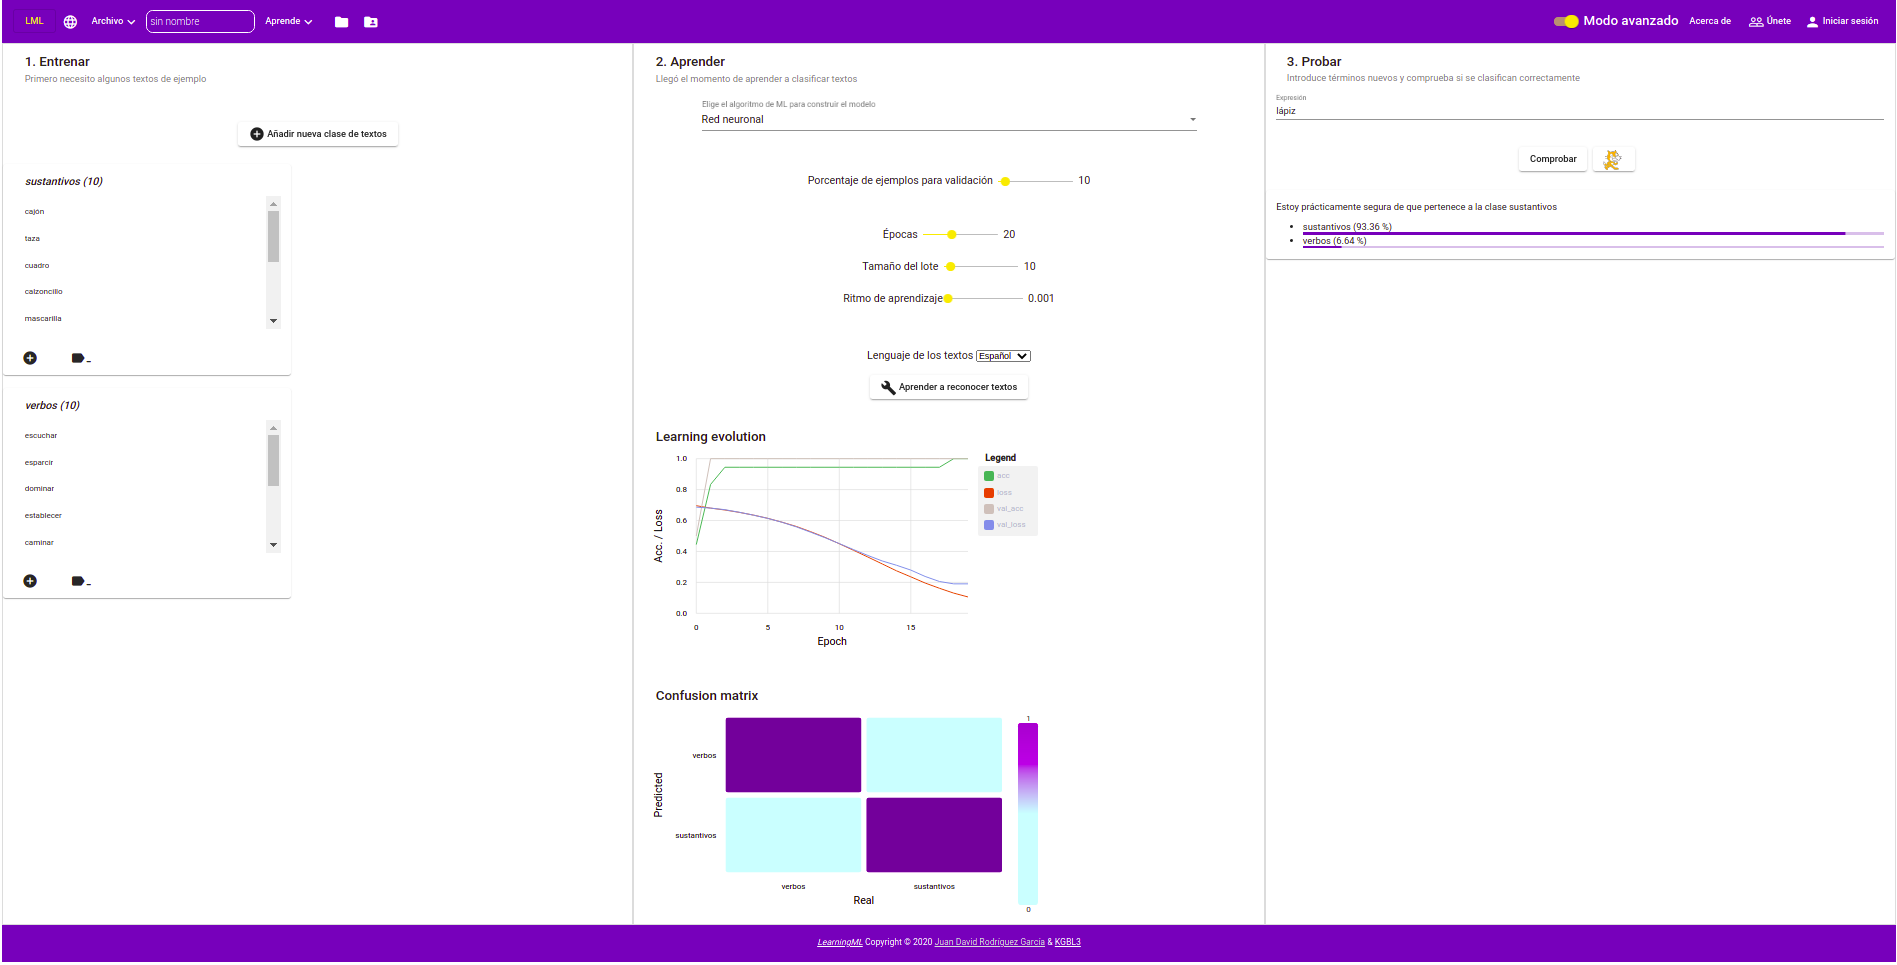
\includegraphics[width=12cm, keepaspectratio]{img/reconocimiento-textos.png}
	\caption{Ejemplo de reconocimiento de textos, diferenciación entre verbos y sustantivos.}\label{fig:reconocimiento-textos}
\end{figure}

\begin{figure}
	\centering
	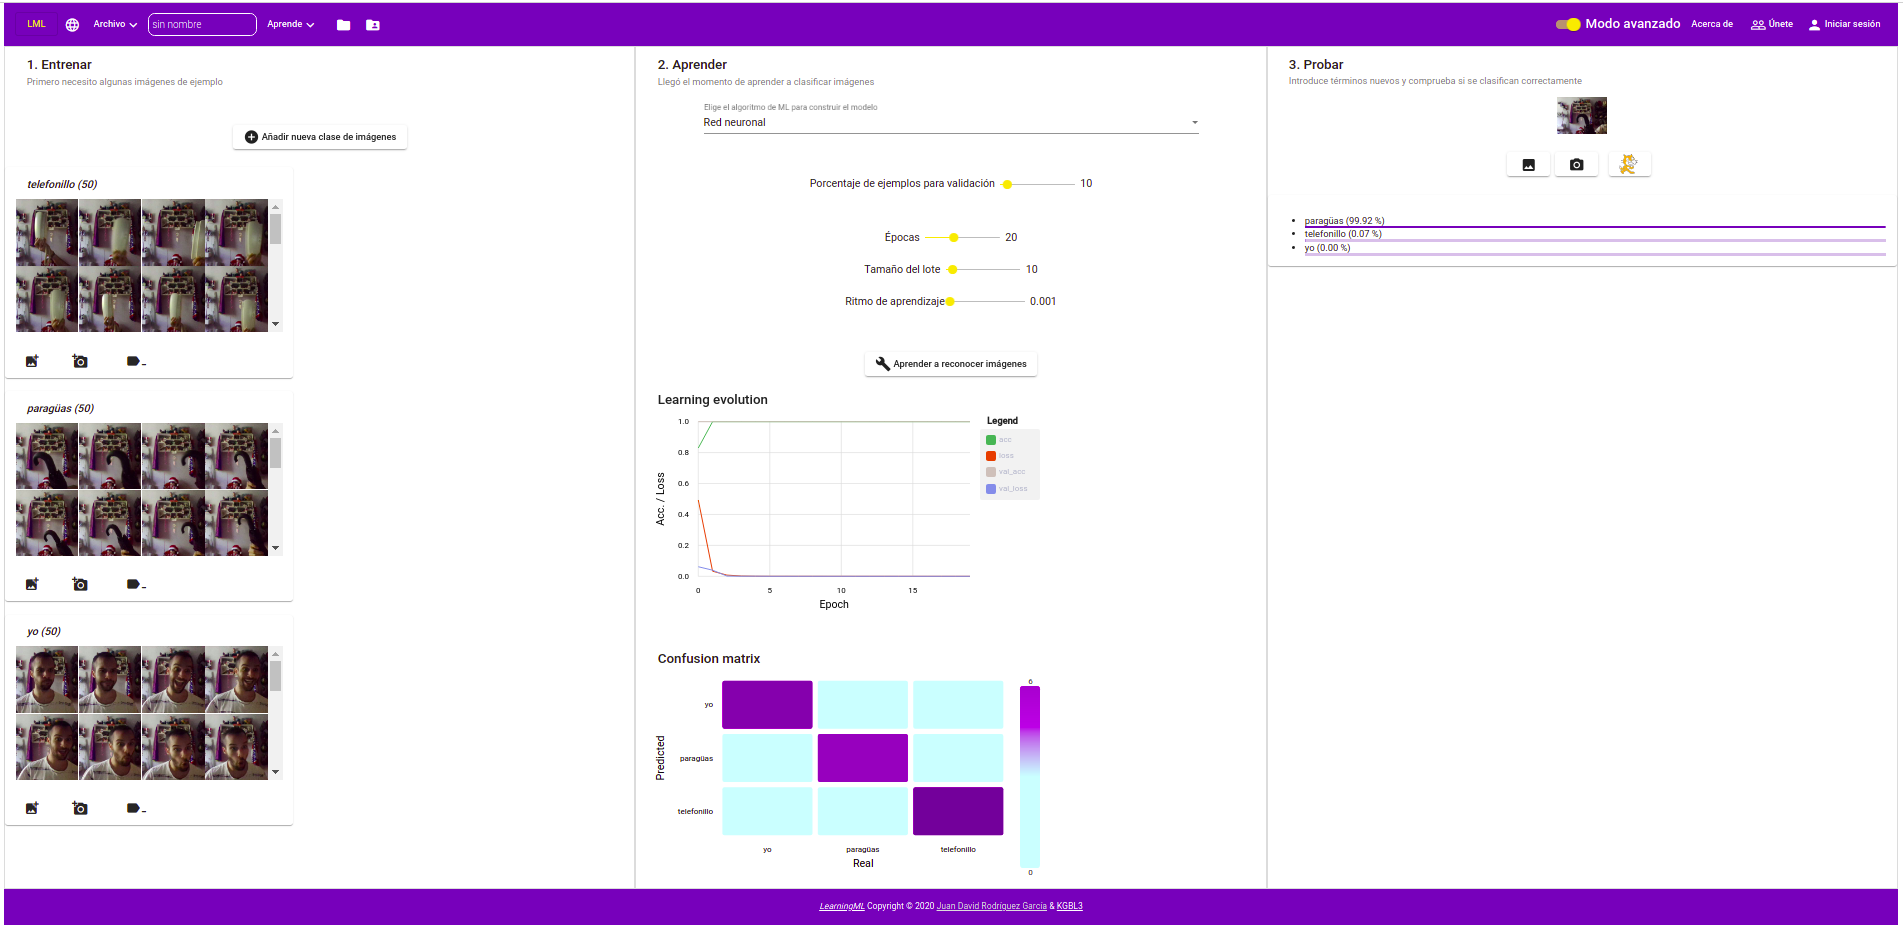
\includegraphics[width=12cm, keepaspectratio]{img/reconocimiento-imagenes.png}
	\caption{Ejemplo de reconocimiento de imagenes, diferenciación entre mi cara, un paragüas y un telefonillo.}\label{fig:reconocimiento-imagenes}
\end{figure}

Además, la aplicación permite al usuario realizar un registro, una vez realizado el registro, el usuario podrá guardar los modelos creados en la nube. En caso de no estar registrado, se permite al usuario realizar una descarga del modelo en formato JSON, de igual manera se permite también cargar un modelo creado con anterioridad.

Dispone también de varios enlaces a tutoriales\footnote{\url{https://web.learningml.org/videotutoriales/}} y al manual de usuario\footnote{\url{https://web.learningml.org/manual-de-learningml/}} en la pestaña \texttt{Aprende}, que resulta muy útil en el caso de que sea la primera visita que se realiza a la página.

Por último destacar que el modelo no solo se puede importar en formato JSON, sino que también permite la exportación del modelo a \texttt{Scratch}\footnote{\url{https://scratch.mit.edu/}}.


\section{HTML 5} 
\label{sec:html5}

\texttt{HTML} (\textit{HyperText Markup Language})~\cite{mdnhtml} es un lenguaje de marcado que se usa para especificar la estructura de una página web.

Los documentos de \texttt{HTML} están escritos en texto plano, se estructuran con diversos elementos y cada elemento está encerrado entre dos parejas de etiquetas~\cite{mdnhtml}, la estructura global de un documento en \texttt{HTML} se compone de las siguientes etiquetas~\cite{gauchat2012gran}:

\begin{itemize}
	\item \textbf{\texttt{<!DOCTYPE>}:} Debe de estar en la primera línea del fichero \texttt{HTML}.
	\item \textbf{\texttt{<html>}:} Se utiliza para comenzar la estructura, esta etiqueta se corresponde con la raíz de la estructura tipo árbol de \texttt{HTML}.
	\item \textbf{\texttt{<head>}:} Se encarga de facilitar información general del documento (título, set de caracteres, \ldots), también se encuentran las etiquetas correspondientes a los archivos externos (\textit{JavaScript}, \textit{CSS3}).
	\item \textbf{\texttt{<body>}:} Se trata del cuerpo del fichero, en él se encuentran todas las etiquetas que dan forma a una página web.
\end{itemize}

\texttt{HTML5} es la última versión de este lenguaje, respecto de la versión anterior incorpora nuevas etiquetas, como \texttt{<header>}, \texttt{<nav>}, \texttt{<section>}, \texttt{<footer>}; así como una mejora en los formularios, \texttt{<form>} añadiendo validaciones, nuevos campos y nuevos atributos. Además dispone de multitud de \texttt{APIs}, que permiten la reproducción de contenido multimedia (etiquetas \texttt{<audio>} y \texttt{<video>}), el almacenamiento de datos en el lado cliente cuando la sesión se encuentra activa (\textit{Web Storage}), \texttt{<canvas>} que permite realizar dibujos o animaciones y la geolocalización, que permite la muestra e interacción de un mapa de \textbf{Google Maps} en la página web.

\section{CSS3}
\label{sec:css3}

\texttt{CSS} (\textit{Cascading Style Sheets})~\cite{mdncss} es el lenguaje utilizado para establecer estilos en los documentos \texttt{HTML}. Describe cómo debe de hacerse el renderizado del elemento al que se haga referencia~\cite{mdncss}.

\texttt{CSS} es uno de los lenguajes base de la \textit{Open Web} y sus especificaciones están estandarizadas por parte de W3C. Con la llegada de \texttt{CSS3} se incrementó el alcance de las especificaciones, lo que provocó que fuese más efectivo crear y desarrollar módulos en esta versión que en las anteriores.

\section{TypeScript}
\label{sec:typescript}

\texttt{TypeScript}~\cite{typescript} es un lenguaje de programación de código abierto desarrollado por \textit{Microsoft} a partir de \texttt{JavaScript}, añadiendo a este lenguaje nueva sintaxis y tipos, lo que convierte a \texttt{TypeScript} en un superconjunto de \texttt{JavaScript}.

Este lenguaje nació en 2012 a partir de la necesidad de mejora de \texttt{JavaScript}, ya que construir una aplicación a gran con este lenguaje era de una complejidad muy alta. Se trata por ende de un lenguaje bastante útil, ya que mantiene las herramientas incorporadas en \texttt{JavaScript ES6}, además de incorporar un tipado estático para evitar errores en tiempo de ejecución y al añadir objetos basados en clases hace que sea mucho más sencillo utilizar programación orientada a objetos, haciéndola más funcional.

\section{Node.js}
\label{sec:nodejs}

\texttt{Node.js}~\cite{nodejs} es un entorno de ejecución de \texttt{JavaScript} orientado al manejo de eventos asíncronos creado por Ryan Dahl en 2009.\\
En el lado cliente el \textit{browser} se encarga de interpretar el código de \texttt{JavaScript}, de la misma manera en el lado servidor, \texttt{Node.js} se encarga de facilitar un entorno de ejecución haciendo uso del motor V8 de \textit{Google}.

Al estar orientado al manejo de eventos asíncronos, \texttt{Node.js} puede soportar una gran cantidad de solicitudes. Al contrario de lo que ocurre en los modelos de concurrencia más comunes, que añaden un nuevo hilo a cada una de las conexiones que llegan, provocando que si se tienen muchas solicitudes sean necesarios muchos servidores; \texttt{Node.js} emplea un único hilo, que itera sobre un bucle de eventos asíncronos, haciendo que cada una de las nuevas peticiones sean un nuevo evento dentro de este bucle, consiguiendo así que el flujo de trabajo no quede bloqueado.

\section{Angular}
\label{sec:angular}

\texttt{Angular}~\cite{angularjs} es un \textit{framework} de código abierto creado por \textit{Google} que permite, haciendo uso de \texttt{HTML} y \texttt{TypeScript}, crear aplicaciones web de una única página, conocidas como SPA (\textit{Single Page Application}).

Una de las ventajas de utilizar \texttt{Angular}, así como de todas las SPA, es la alta velocidad de carga entre las distintas vistas que pueda tener la aplicación web, ya que al cambiar de vista no se recarga la página.

Las versiones de este \textit{framework} han ido evolucionando, la primera fue \texttt{AngularJS}, en 2010, mientras que las siguientes versiones han ido evolucionando desde \texttt{Angular2}, la segunda versión. La versión más reciente es de mayo de 2021, \texttt{Angular12}.

Una aplicación de \texttt{Angular} utiliza cuatro clases distintas, que se comunican entre ellas usando decoradores, que se encargan de cargar únicamente los metadatos que necesita esa clase. Las clases que utiliza \texttt{Angular} son:

\begin{itemize}
	\item \textbf{Módulos}: Definen los componentes que van a formar la aplicación, así como las dependencias y los servicios. El módulo principal suele nombrarse como \texttt{AppModule}, y es el que contiene el sistema de arranque de la propia aplicación. Gracias a esta organización la carga inicial es mínima, ya que los módulos se cargan únicamente cuando vayan a ser utilizados.
	\item \textbf{Componentes}: Contienen la lógica y los datos de la propia aplicación, controlan las plantillas que se cargan al cambiar la \texttt{URL}, conformando la interfaz de usuario. Los componentes pueden tener a su vez uno o varios subcomponentes, que se relacionan entre sí usando eventos, para actualizar datos, o usando propiedades, que modifican las plantillas escritas en \texttt{HTML} conformando las vistas. Una clase se define como Componente usando el decorador @Component.
	\item \textbf{Servicios}: Se componen de los datos o funcionalidades generales, que no forman parte de ninguna vista específicamente. Se usan para intercambiar datos entre componentes. Para definir una clase como Servicio se utiliza el decorador @Injectable.
	\item \textbf{Directivas}: Definen los términos claves que utilizan las plantillas. Hay dos clases de directivas:
	\begin{itemize}
		\item Directiva de atributo: Modifica el comportamiento del componente.
		\item Directiva estructural: Modifica la apariencia.
	\end{itemize}
\end{itemize}

\subsection{MVC}
\label{subsec:mvc}

\texttt{MVC} (\textit{Modelo Vista-Controlador})~\cite{mvc}, es el patrón que se utiliza en \texttt{Angular} a la hora de desarrollar una aplicación. Los elementos que lo conforman son:

\begin{itemize}
	\item \textbf{Modelo}: Se encarga de representar y tratar los datos de la aplicación, manejando las consultas y acciones de la base de datos, si la tuviera. 
	\item \textbf{Vista}: Se encarga del diseño de la interfaz de usuario, haciendo que el Modelo y el Controlador no se tengan que hacer cargo de esa parte.
	\item \textbf{Controlador}: Recibe los eventos de entrada, se comunica con el Modelo, obtiene las vistas que sean necesarias y produce una salida como respuesta a ese evento.
\end{itemize}

Esta arquitectura tiene varias ventajas sobre otro tipo de arquitecturas del mismo tipo ya que mejora la estabilidad, separando cada tipo de lógica, facilita el mantenimiento y posibilita el uso de componentes.

\subsection{CLI}
\label{subsec:cli}

\texttt{Angular CLI} (\textit{Command Line Interface})~\cite{angularcli} es una herramienta de línea de instrucciones creada por los desarrolladores de \texttt{Angular}. Contiene herramientas que se pueden utilizar para el mantenimiento y desarrollo de aplicaciones, entre estas herramientas destacan el compilador, el sistema de testing y el servidor web. Gracias a estas herramientas predefinidas se puede crear el esqueleto básico de una aplicación en \texttt{Angular} de una manera muy sencilla, así como los nuevos componentes, servicios o directivas que forman la aplicación.

\section{TensorFlow}
\label{sec:tensorflow}

\texttt{TensorFlow}~\cite{tensorflow} es un sistema de aprendizaje automático creado por \textit{Google Brain}, es una plataforma que permite construir y entrenar redes neuronales de una manera muy eficiente y completa.. En 2015 \texttt{TensorFlow} pasó a ser \textit{software libre}, por lo que todo el mundo puede utilizarlo en sus aplicaciones, así como modificarlo siempre que fuera necesario.

\subsection{MobileNets}
\label{subsec:mobilenets}

\texttt{MobileNets} es una biblioteca de \texttt{TensorFlow}, así como una red neuronal convolucional, que es mucho más eficiente ya que únicamente utiliza una capa convolucional de la dimensión deseada con un único filtro.

Esta biblioteca es utilizada por el reconocimiento de imágenes.

\section{Análisis de audio}
\label{sec:analisis-audio}

El análisis de señales de audio~\cite{gonzalez2019analisis} es un tema importante en los tiempos que vivimos. La tecnología actual nos da la posibilidad de crear sistemas de reconocimiento de señales de audio eficientes en entornos semánticos restringidos. El proceso de extracción de características no supervisado supone un avance en este campo, ya que reduce el error en la clasificación de fonemas.

\subsection{Web Audio API}
\label{subsec:audio-api}

Para este proyecto se utilizó la API web de audio~\cite{web-audio-api}, que proporciona un sistema potente y versátil para controlar el audio, permitiendo a los desarrolladores elegir fuentes de audio, agregar efectos, crear visualizaciones y mucho más.

Las operaciones de audio básicas están dentro de un \texttt{AudioContext} y se realizan mediante \texttt{AudioNodes}, que están vinculados entre sí para formar un gráfico de enrutamiento de audio. Dentro de un mismo context se pueden usar varias fuentes.

Un proyecto simple usando esta herramienta tendría la siguiente forma:

\begin{enumerate}
	\item Crear contexto de audio.
	\item Dentro del contexto, se crean fuentes.
	\item Se crean nodos de efectos, como reverberación, filtro biquad, panoramizador, compresor...
	\item Elegir el destino final del audio, por ejemplo, los altavoces.
	\item Conecte las fuentes a los efectos y los efectos al destino.
\end{enumerate}

\begin{figure}
	\centering
	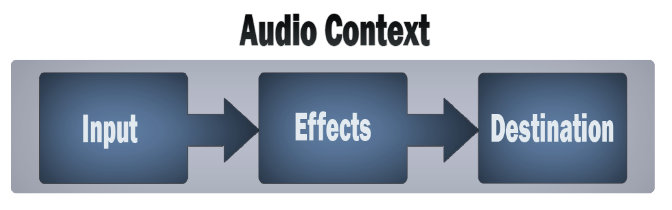
\includegraphics[width=9cm, keepaspectratio]{img/web-audio-api.png}
	\caption{Análisis de audio con la API web de audio.}\label{fig:audio-api}
\end{figure}

No obstante, en este proyecto no se crearon nodos de efecto, ya que los datos que se necesitaban eran los datos en bruto.

Para obtener los datos se usó la interfaz de \texttt{AnalyserNode}~\cite{analyser-node}, en particular la función \texttt{getByteFrequencyData()}, que guarda los datos obtenidos en frecuencia en un array previamente creado.

%%%%%%%%%%%%%%%%%%%%%%%%%%%%%%%%%%%%%%%%%%%%%%%%%%%%%%%%%%%%%%%%%%%%%%%%%%%%%%%%
%%%%%%%%%%%%%%%%%%%%%%%%%%%%%%%%%%%%%%%%%%%%%%%%%%%%%%%%%%%%%%%%%%%%%%%%%%%%%%%%
% DISEÑO E IMPLEMENTACIÓN %
%%%%%%%%%%%%%%%%%%%%%%%%%%%%%%%%%%%%%%%%%%%%%%%%%%%%%%%%%%%%%%%%%%%%%%%%%%%%%%%%

\cleardoublepage
\chapter{Diseño e implementación}
\label{chap:diseño-implementacion}

\section{Arquitectura general} 
\label{sec:arquitectura}

La arquitectura de \texttt{LearningML} está basada en el modelo MVC~\cite{mvc}. Es una arquitectura que está muy bien desarrollada y preparada para que, en el caso de querer realizar cambios, los desarrolladores no tengan muy complicado el añadir funcionalidades.

En la figura~\ref{fig:arquitectura} podemos ver cómo está organizada aplicación: Primero se crea el modelo, escogiendo el tipo de extracción de características que se van a realizar, así como el algoritmo que se va a utilizar. El servicio \texttt{labeled-data-manager} se encarga de manejar todos los cambios y de guardar las características que definen al modelo, como el tipo de análisis que vamos a realizar o el algoritmo que se utiliza.

Después de elegir el tipo de análisis y el algoritmo, el modelo procede a analizar todas las muestras que se han añadido, este análisis se realiza con el servicio \texttt{FeatureExtraction}, que a su vez tiene dos servicios debajo suya: \texttt{FeatureExtractorText} y \texttt{FeatureExtractorImage}.

Cada uno de ellos se encarga de realizar la extracción de características del modelo, atendiendo al tipo de datos que se le van a introducir.

Una vez se han extraído los datos, se procede a crear el modelo. La creación se produce en el fichero \texttt{ml-model}, que haciendo uso de la función \texttt{train()} se encarga de coger el array de datos y entrenar al modelo para el reconocimiento, teniendo en cuenta el tipo de algoritmo utilizado.

Por último, cuando el modelo ya está entrenado, dependiendo del tipo de análisis que se haya querido realizar, hace uso de los ficheros \texttt{ml-test-image-model} o \texttt{ml-test-text-model} para poder realizar pruebas.

\begin{figure}
	\centering
	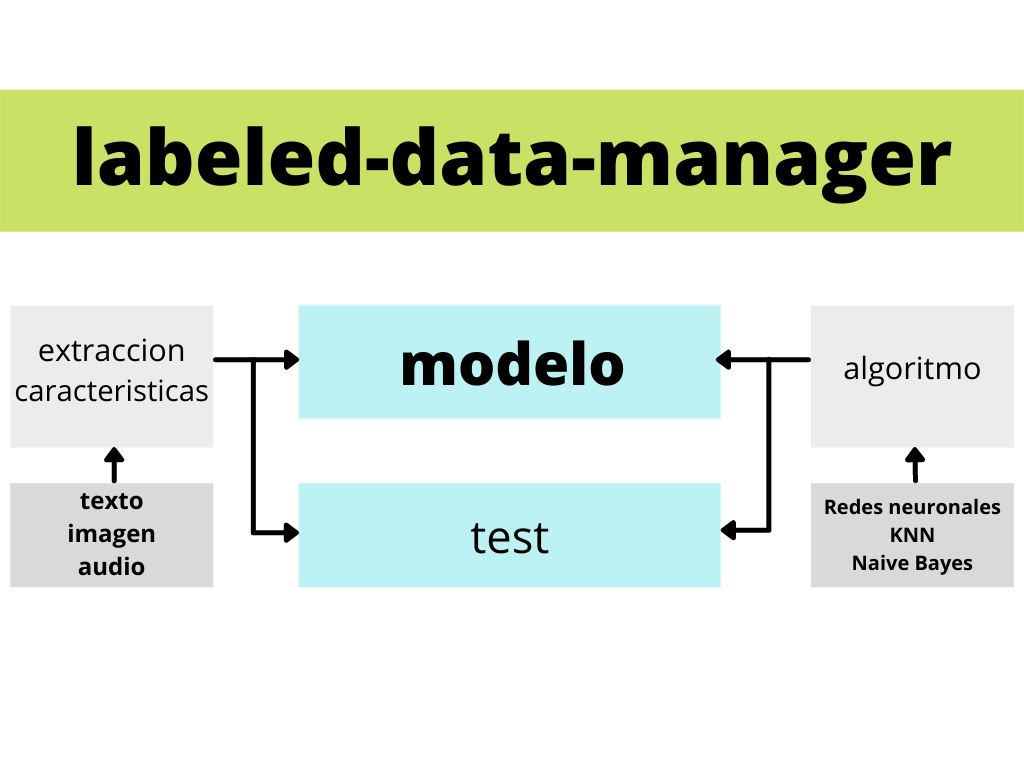
\includegraphics[width=11cm, keepaspectratio]{img/arquitectura-learningml.png}
	\caption{Estructura de la arquitectura de \texttt{LearningML}.}\label{fig:arquitectura}
\end{figure}

\section{Cambio en la arquitectura}
\label{sec:cambio-arquitectura}

El principal cambio que debía hacer en la arquitectura era añadir un nuevo componente, \texttt{ml-test-sound-model}, así como añadir en el fichero \texttt{interfaces} los tipos que iba a utilizar, también fue necesario añadir un nuevo servicio, \texttt{feature-extractor-sound}, que se encargaría de analizar los datos de audio recibidos y extraer las características que se fueran a utilizar.

El cambio en la arquitectura no fue muy complicado, ya que la aplicación estaba preparada para poder realizar cambios de esta índole sin realizar un esfuerzo muy grande.

Además había que encontrar la manera de recoger el audio directamente del micrófono para su posterior análisis, para ello había dos posibilidades:
\begin{itemize}
	\item Utilizar el analizador de audio de Angular, que facilitaba aspectos como la introducción en el código.
	\item Utilizar el analizador de audio de la API web, del que se obtenían los datos de una manera más sencilla.
\end{itemize}

Finalmente, me decidí por usar la API web para el audio, ya que los datos que llegaban eran más sencillos de interpretar.

\section{Cambio en la interfaz}
\label{sec:cambio-interfaz}

En cuanto a la interfaz de usuario no hubo que realizar muchos cambios:
\begin{itemize}
	\item En el fichero \texttt{ml-home} se añadió un ``container'' para el audio, como se puede ver en la figura~\ref{fig:main-page}.
	\item En el fichero \texttt{ml-model} bastó con añadir la etiqueta del componente \texttt{ml-test-sound-model}, además de añadir una entrada de texto que se utilizaría para pedir al usuario la duración de los audios, como se puede ver en la figura~\ref{fig:audio-page}.
\end{itemize}

Además, por supuesto, del fichero \texttt{ml-test-sound-model}, que siguiendo la estructura de los otros ficheros de test, no fue una tarea muy complicada de realizar.

\begin{figure}
	\centering
	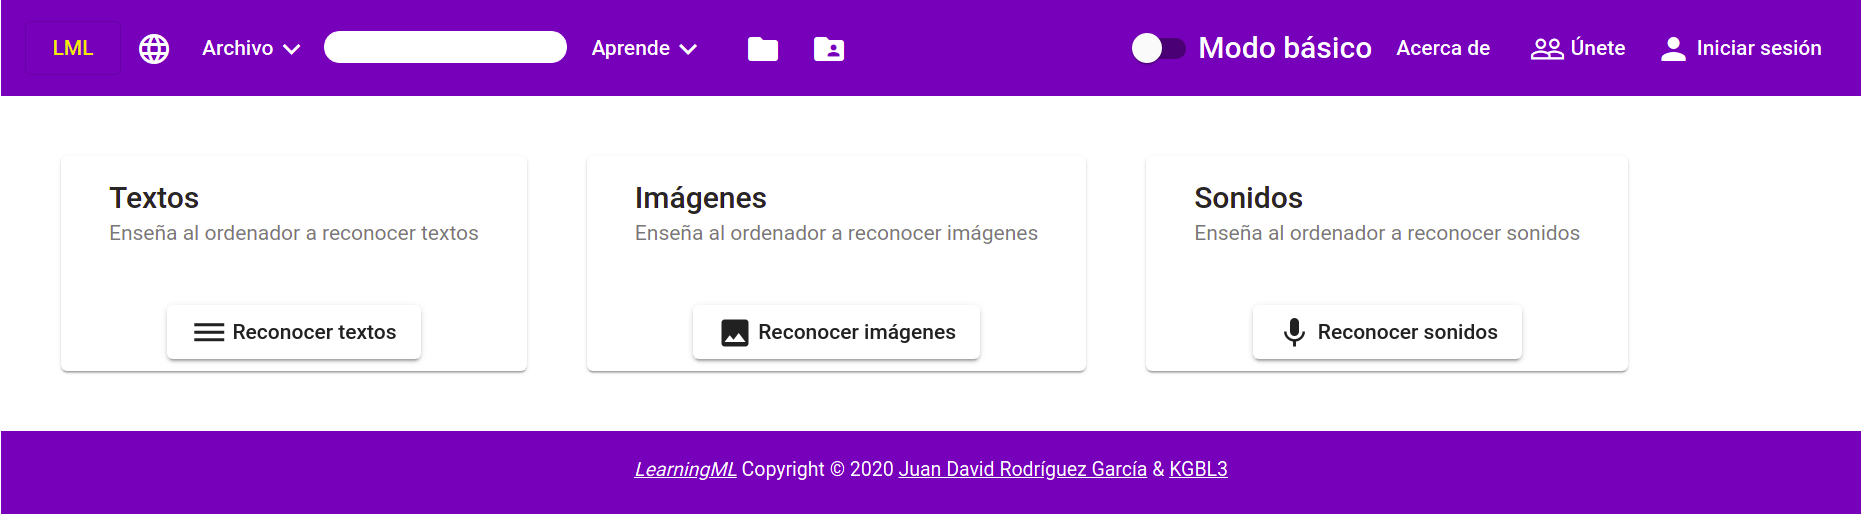
\includegraphics[width=15cm, keepaspectratio]{img/pagina-principal.png}
	\caption{Página principal de \texttt{LearningML}.}\label{fig:main-page}
\end{figure}

\begin{figure}
	\centering
	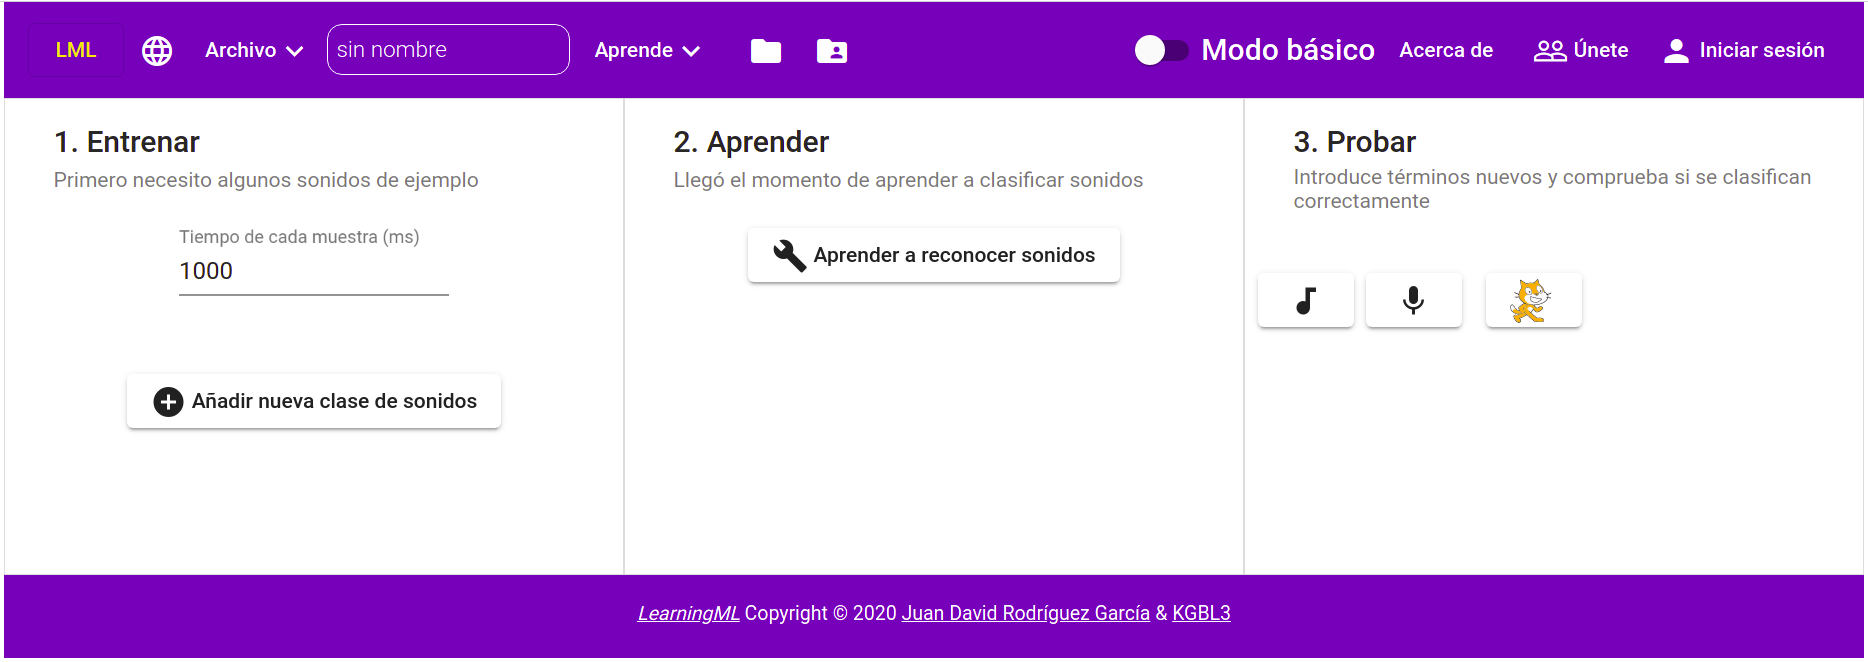
\includegraphics[width=15cm, keepaspectratio]{img/audio-model.png}
	\caption{Página de análisis de un modelo de audio en \texttt{LearningML}.}\label{fig:audio-page}
\end{figure}

\section{Componente micrófono}
\label{sec:mic}

El componente principal, sobre el que gira toda la obtención de elementos de audio es el micrófono. Este elemento se creó como un nuevo componente al que se llamó \texttt{ml-microphone}. Este componente sería el encargado de recoger el audio directamente del micrófono del usuario y enviárselo al modelo para que pueda trabajar con él. La arquitectura del componente debía de ser similar a la que tenían otros componentes que hacían un trabajo similar al suyo pero para otros tipos de análisis, como \texttt{ml-web-cam} hace para el análisis de imágenes. Por tanto, había una serie de funciones que debían de aparecer:
\begin{itemize}
	\item Una función para activar el micrófono, \texttt{enableAudio()}.
	\item Una función para desactivar el micrófono, \texttt{disableAudio()}.
	\item Una función para mostrar o esconder el micrófono, \texttt{toggleMic()}.
	\item Una función para comenzar las grabaciones, \texttt{startRecording()}.
	\item Una función para terminar las grabaciones, \texttt{stopRecording()}.
	\item Una función para capturar y enviar los datos obtenidos al propio modelo, \texttt{captureAudio()}.
\end{itemize}

Además debía de tener varios eventos: i) para indicar cuándo se cerraba el micrófono, ii) para enviar los datos al modelo y iii) para enviar los datos cuando se estaba probando, es decir, una vez el modelo ya estaba creado.

\subsection*{enableAudio()}

Es la función encargada de pedir los permisos al navegador para poder utilizar el micrófono, esto se hace mediante el siguiente código:

{\footnotesize
\begin{verbatim}
	navigator.mediaDevices.getUserMedia({ video: false, audio: true })
	.then((stream) => {
		//
	});
\end{verbatim}
}

Después de pedir los permisos, se procede a crear todas las variables que vamos a necesitar para poder realizar el análisis de audio, teniendo en cuenta una variable booleana, \texttt{testing}, que indica si queremos capturar estos audios para test o para crear el modelo.

\subsection*{disableAudio()}

Es la función encargada de deshabilitar la captura de audio, para ello comienza por parar todas las posibles pistas que haya activas mediante el siguiente código:

{\footnotesize
\begin{verbatim}
	this.localstream.getTracks().forEach((element: any) => {
		element.stop();
	});
\end{verbatim}
}

Una vez se hayan detenido todas las pistas, se reinician las variables que se habían creado en \texttt{enableAudio()}.

\subsection*{startRecording()}

Es la función que se encarga de comenzar a grabar, para que la grabación se realice periódicamente teniendo en cuenta el valor que haya introducido el usuario, se hace uso de la función \texttt{interval} y se realiza una subscripción. Las subscripciones se usan para que cada vez que la función \texttt{interval} devuelva un valor, se ejecute un código personalizado, escogido por el desarrollador, para este caso, simplemente se hará una llamada a la función \texttt{captureAudio()}.

\subsection*{stopRecording()}

Es la función encargada de terminar la grabación, para ello primero deshabilita el micrófono, haciendo una llamada a \texttt{disableAudio()}, para después limpiar el intervalo creado con la función \texttt{interval} y anular la subscripción. Por último colocará la variable \texttt{testing} en su valor original y hará uso del evento \texttt{onCloseMic} para informar que la grabación ha terminado.

\subsection*{captureAudio()}

Es la función más importante, ya que se encarga de recoger los datos y enviarlos.

Primero se crea una fuente, haciendo uso de la función \texttt{createMediaStreamSource()} de la interfaz \texttt{AudioContext}, después se conecta esta fuente al analizador, que haciendo uso de la función \texttt{getByteFrequencyData()} guardará los datos de frecuencias obtenidos en la variable \texttt{dataArray}.

Una de las pegas que puede tener este tipo de análisis es que la primera muestra siempre llega con todos los valores a cero, independientemente de si se graba o no, como que una muestra sea igual en todas las etiquetas podría confundir al modelo. Después de guardar los datos en la variable \texttt{dataArray}, se comprueba si la media es cero, en el caso de que lo sea, se omite esa muestra.

Después de realizar las comprobaciones pertinentes, el siguiente paso será enviar los datos, pero para ello es necesario saber si se van a enviar para test o para la creación del modelo. Por ello haciendo uso de la variable booleana \texttt{testing} escogemos uno de los dos posibles eventos para enviar los datos. Además en el caso de que las muestras se vayan a usar en la creación del modelo crearemos un nuevo elemento de audio para añadir al ``container'' con el resto de elementos.

Finalmente, se reinician los valores de la variable \texttt{dataArray}.

\section{Obtención de datos}
\label{sec:obtencion-datos}

La obtención de datos se realiza en el fichero \texttt{feature-extractor-sound}.

\subsection{Intercambio de datos entre componentes}
\label{subsec:intercambio-datos}

Llegado el momento del envío de los datos desde el fichero \texttt{ml-microphone-component} hacia \texttt{feature-extractor-sound}, se produjo uno de los primeros problemas que se deberían solucionar: el intercambio de datos entre componentes, la función que se encargará de controlar este intercambio será \textit{extractInstanceFeatures}.

Este intercambio se realiza mediante eventos, los eventos se encargan de ``emitir'' una trama de datos desde un componente a otro, en este intercambio lo ideal hubiera sido que la muestra se enviara tal como se recoge, es decir un array de dos dimensiones con los datos como números enteros, pero al hacer el envío de esa manera la aplicación únicamente reconocía una muestra, para evitar este error se decidió crear un tipo determinado para las muestras: el tipo \texttt{AudioData}. Después de varias pruebas, cambiando el tipo de dato desde el array de números enteros inicial hasta un objeto en \texttt{JSON} con una estructura determinada, se llegó a la conclusión de que lo más óptimo era convertir el array en una cadena de caracteres, \texttt{string}, para su posterior envío.

Una vez se había realizado el envío, y se comprobó que el número de muestras crecía, hubo que enfrentarse al siguiente problema: el análisis de los datos recibidos.

\subsection{Análisis de datos}
\label{subsec:analisis-datos}

Este análisis podía acarrear algún problema, ya que los datos llegaban como una cadena de caracteres, pero para la predicción y la extracción de características era necesario que los datos fueran de nuevo un array de números enteros, para convertir la cadena de caracteres en un array de números enteros se decidió crear una nueva función que se encargaría de hacerlo: \textit{string2number}, que recibiría la cadena de caracteres y devolvería un tensor de una dimensión con los datos convertidos.

Con el problema del intercambio de datos solucionado, el siguiente paso consistía en analizar de manera correcta e inequívoca los datos. Para ello primero se decidió pasar por una ventana de Hamming el array de datos, la ventana de Hamming se utiliza para realizar filtrados en señales de audio, dando una menor importancia a los datos del principio y del final de la muestra y haciendo que los datos de la zona intermedia tomen una mayor importancia.

\begin{figure}
	\centering
	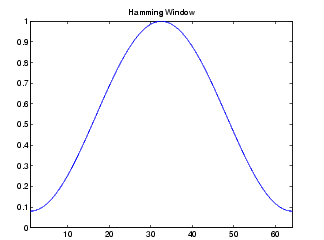
\includegraphics[width=12cm, keepaspectratio]{img/hamming-window.png}
	\caption{Ventana de Hamming.}\label{fig:hamming-window}
\end{figure}

\subsection{Extracción de datos de interés}
\label{subsec:extraccion-datos}

Para la extracción de datos de interés únicamente se introdujeron los datos obtenidos por el micrófono y filtrados por la ventana de Hamming, pero añadir los datos tenía un problema. Y es que todas las muestras tenían una larga cola de ceros al final, algo que confundía al modelo y hacía que las predicciones no fueran buenas, véase la figura~\ref{fig:silbido1024}.

\begin{figure}
	\centering
	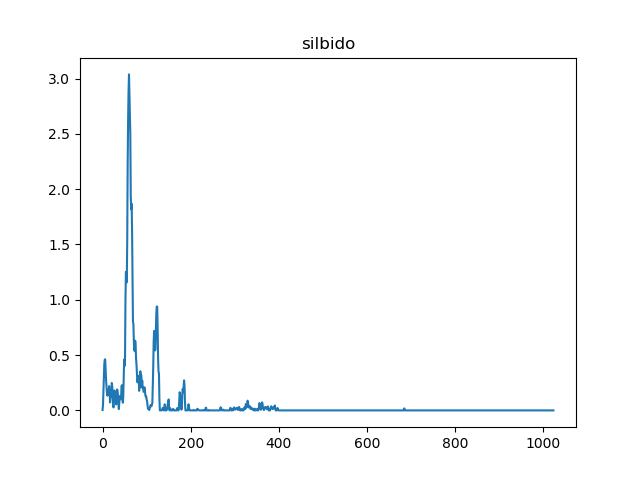
\includegraphics[width=12cm, keepaspectratio]{img/silbido1024.png}
	\caption{Valores de la FFT de un silbido con 1024 muestras.}\label{fig:silbido1024}
\end{figure}

Para evitar confusiones de este estilo, los datos recibidos debían de recortarse, para omitir la larga cola de ceros y quedarse únicamente con los datos de las frecuencias que tienen valores altos. Pero la dificultad estaba en elegir bien el valor a partir del cual se iba a cortar, ya que si se cortaba demasiado pronto podrían quedarse muy pocas muestras y si se hacía demasiado tarde escogería aún una pequeña cola de ceros.

Por ello, se realizaron pruebas cortando a varias longitudes, y se llegó a la conclusión de que lo mejor sería cortar por la zona media, es decir, en 512 muestras, como se puede observar en la figura~\ref{fig:silbido512}.

\begin{figure}
	\centering
	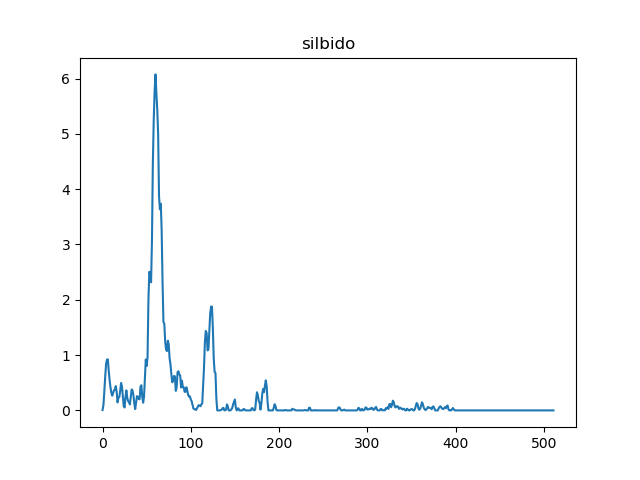
\includegraphics[width=12cm, keepaspectratio]{img/silbido512.png}
	\caption{Valores de la FFT de un silbido con 512 muestras.}\label{fig:silbido512}
\end{figure}

\section{Adición de nuevas muestras en el conjunto de datos del modelo}
\label{sec:adicion-datos}

Después de haber obtenido todos los valores de las muestras, el siguiente paso consistía en añadir estos nuevos datos al conjunto de datos principal del modelo.

La función \textit{addLabeledAudio} recibe como parámetro de entrada un objeto con la siguiente estructura \texttt{\{label, data\}}, y es la encargada de añadir estos datos, siguiendo tres pasos:

\begin{itemize}
	\item Primero se encarga de comprobar si la etiqueta con la que viene la muestra está dentro de las etiquetas conocidas por el modelo, para ello hace uso de la función \textit{indexOf}, que devolvería un -1 en el caso de que la etiqueta no fuese reconocida por parte del modelo.
	\item Después hará uso de la función \textit{extractInstanceFeatures}, que se ha explicado en las subsecciones~\ref{subsec:intercambio-datos},~\ref{subsec:analisis-datos} y~\ref{subsec:extraccion-datos}. Al tratarse de programación asíncrona, se utiliza la función \textit{then} cuya función consiste en esperar a que la función asíncrona devuelva un valor para después hacer uso de ese valor.
	\item Por último, haciendo uso del valor devuelto por la función \textit{extractInstanceFeatures}, añade el nuevo dato al conjunto del modelo.
\end{itemize}

\section{Creación del conjunto de datos}
\label{sec:creacion-dataset}

Se trata de nuevo de una función asíncrona, \textit{buildDataset}, que se encarga de coger los datos del modelo y crear un conjunto de datos con el que se pueda trabajar. Para ello hace uso de las funciones explicadas en las subsecciones~\ref{subsec:intercambio-datos},~\ref{subsec:analisis-datos}, ~\ref{subsec:extraccion-datos} y en la sección~\ref{sec:adicion-datos}.

Finalmente el conjunto de datos tendría la siguiente estructura:

\begin{verbatim}
	dataset = {
    	data: [],
    	labels: [],
    	dataArray: []
  	};
\end{verbatim}

La clave \textit{data} contiene todos los datos en forma de tensor, mientras que la clave \textit{dataArray} tiene los datos pero en forma de array. Por último la clave \textit{labels} contiene todas las etiquetas que es capaz de reconocer el modelo.

La construcción de este objeto se hace mediante dos bucles que iteran sobre los distintos datos y van utilizando la función \textit{addLabeledAudio} sobre cada uno de ellos.

%%%%%%%%%%%%%%%%%%%%%%%%%%%%%%%%%%%%%%%%%%%%%%%%%%%%%%%%%%%%%%%%%%%%%%%%%%%%%%%%
%%%%%%%%%%%%%%%%%%%%%%%%%%%%%%%%%%%%%%%%%%%%%%%%%%%%%%%%%%%%%%%%%%%%%%%%%%%%%%%%
% EXPERIMENTOS Y VALIDACIÓN %
%%%%%%%%%%%%%%%%%%%%%%%%%%%%%%%%%%%%%%%%%%%%%%%%%%%%%%%%%%%%%%%%%%%%%%%%%%%%%%%%

\cleardoublepage
\chapter{Experimentos y validación}
\label{chap:experimentos-validacion}

Para la validación de un modelo, basta con abrir el inspector en el navegador que se esté utilizando y al crear el modelo comprobar que en la consola los valores que aparecen al lado de la palabra \texttt{Accuracy} sean cercanos a uno, ya que esto indica lo que tarda en llegar a un acierto máximo, uno, en las distintas épocas por las que pasa el modelo.

Un buen modelo podría tener una forma similar a la que se expone en la figura~\ref{fig:validacion}. En esta figura podemos observar la convergencia de los valores de acierto del modelo, que comienzan con un valor bajo, en este caso, de 0,2, y que converge rápidamente alcanzando valores aceptables como son 0,8 y 0,9, hasta que finalmente llega a 1. Cada vez que llega a 1, se cambia de época, y como podemos observar a cada época, se converge más rápido a 1.

\begin{figure}
	\centering
	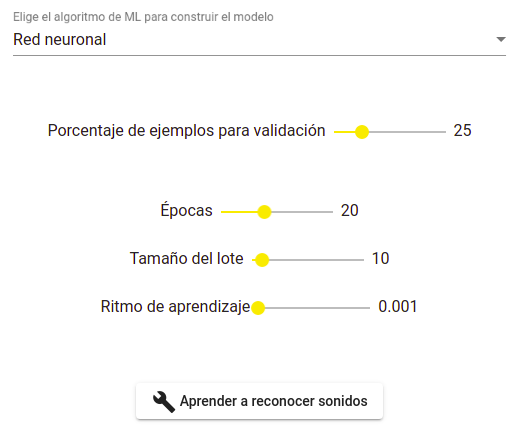
\includegraphics[width=10cm, keepaspectratio]{img/configuracion-25.png}
	\caption{Configuracion del Modo Avanzado.}\label{fig:configuracion}
\end{figure}

Además, gracias a la opción de \textit{Modo Avanzado}, figura~\ref{fig:configuracion}, podemos escoger el porcentaje de datos que se usarán como ejemplos de validación, al cambiar estos valores, aparecen la evolución del aprendizaje, ver figura~\ref{fig:learning-evolution}, y la matriz de confusión, figura~\ref{fig:matriz-confusion}.

\begin{figure}
	\centering
	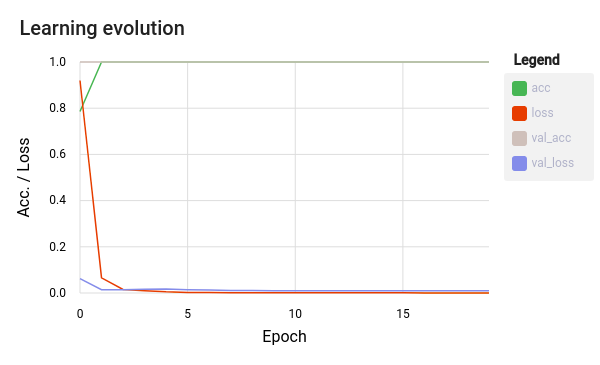
\includegraphics[width=10cm, keepaspectratio]{img/learning-evolution-25.png}
	\caption{Evolución del aprendizaje con un valor del 25\% de ejemplos de validación.}\label{fig:learning-evolution}
\end{figure}

La gráfica de la evolución del aprendizaje nos muestra, quizá de una manera más intuitiva que la figura~\ref{fig:validacion}, el cambio que ha llevado el modelo en cuanto a acierto y error a lo largo de las épocas que se hayan escogido en la configuración del modelo, ver figura~\ref{fig:configuracion}.

\begin{figure}
	\centering
	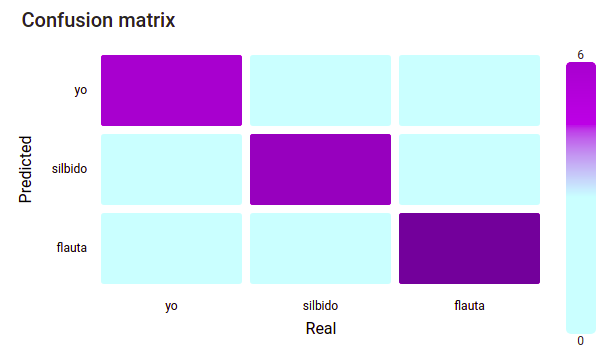
\includegraphics[width=10cm, keepaspectratio]{img/confusion-matrix-25.png}
	\caption{Matriz de confusión con un valor del 25\% de ejemplos de validación.}\label{fig:matriz-confusion}
\end{figure}

La matriz de confusión nos explica en forma de tabla los datos que predice y los que son en realidad. En tonos morados tenemos un mayor valores más altos de ese acontecimiento, por lo que un modelo bien realizado debería de tener la diagonal principal en tonos morados, y el resto en tonos azulados.

%FIXME: desarrollar un poco más qué es lo que se puede ver en la figura.

\begin{figure}
	\centering
	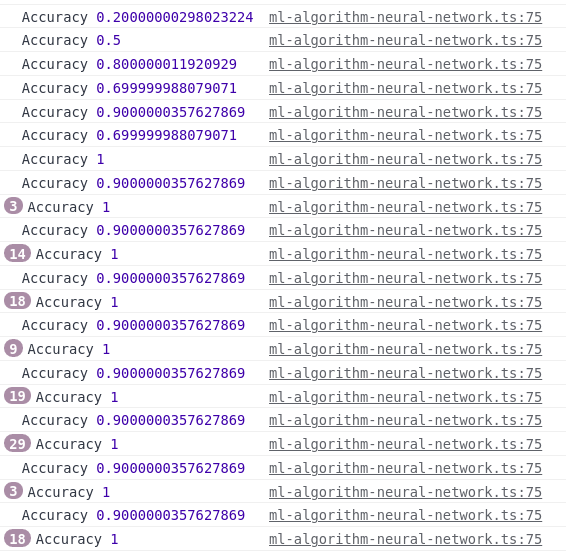
\includegraphics[width=10cm, keepaspectratio]{img/accuracy2.png}
	\caption{Validación de un modelo.}\label{fig:validacion}
\end{figure}

\section{Voz vs. Silbido vs. Flauta}
\label{sec:yo-silv-flauta}

Para este experimento se buscó tres fuentes que tuvieran distinto timbre, para comprobar si la diferenciación era correcta.

Se tomaron muestras de audio de:
\begin{itemize}
	\item Voz: bajo la etiqueta ``yo'', son muestras de audio de yo hablando.
	\item Silbido: con la etiqueta ``silbido'' tenemos muestras de audio de un silbido.
	\item Flauta: en la etiqueta ``flauta'' tenemos muestras del sonido de una flauta dulce con la nota do más grave.
\end{itemize}

Las muestras se tomaron con duración de 1000ms, que es la duración estándar que se decidió colocar. Después se recortaron para dejarlas en 512 muestras, y los resultados obtenidos se pueden observar en las figuras~\ref{fig:silbido},~\ref{fig:yo} y~\ref{fig:flauta}.

%FIXME: explicar algo más en detalle qué se ve en cada una de las figuras

\begin{figure}
	\centering
	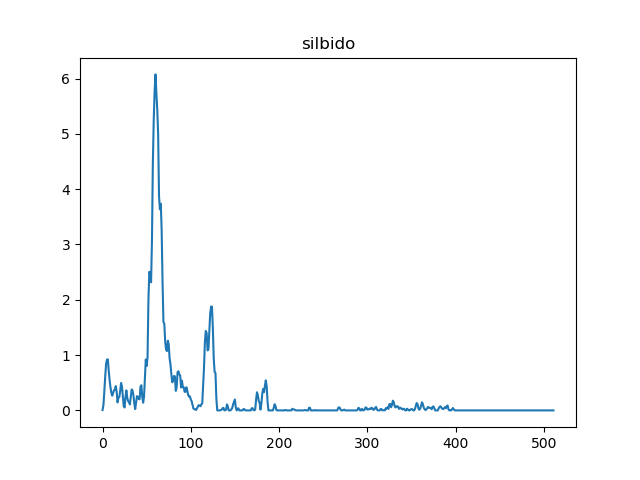
\includegraphics[width=12cm, keepaspectratio]{img/silbido512.png}
	\caption{Valores de la FFT de un silbido con 512 muestras.}\label{fig:silbido}
\end{figure}

En la figura~\ref{fig:silbido} podemos observar un pico bastante alto en las frecuencias bajas y algún armónico, hasta que acaba tendiendo a cero en una zona muy cercana al inicio dela gráfica.

\begin{figure}
	\centering
	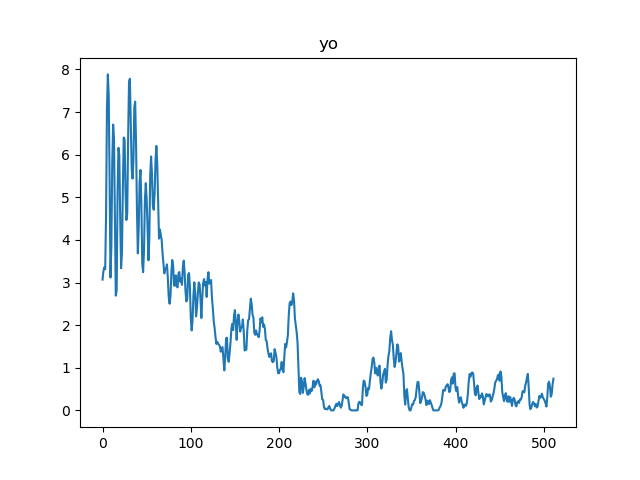
\includegraphics[width=12cm, keepaspectratio]{img/yo512.png}
	\caption{Valores de la FFT de una persona hablando con 512 muestras.}\label{fig:yo}
\end{figure}

En la figura~\ref{fig:yo} observamos que la caída de valores a lo largo de la gráfica es menor, con más subidas y bajadas y picos más exagerados, tiende a cero en las frecuencias finales, que son las que se omiten.

\begin{figure}
	\centering
	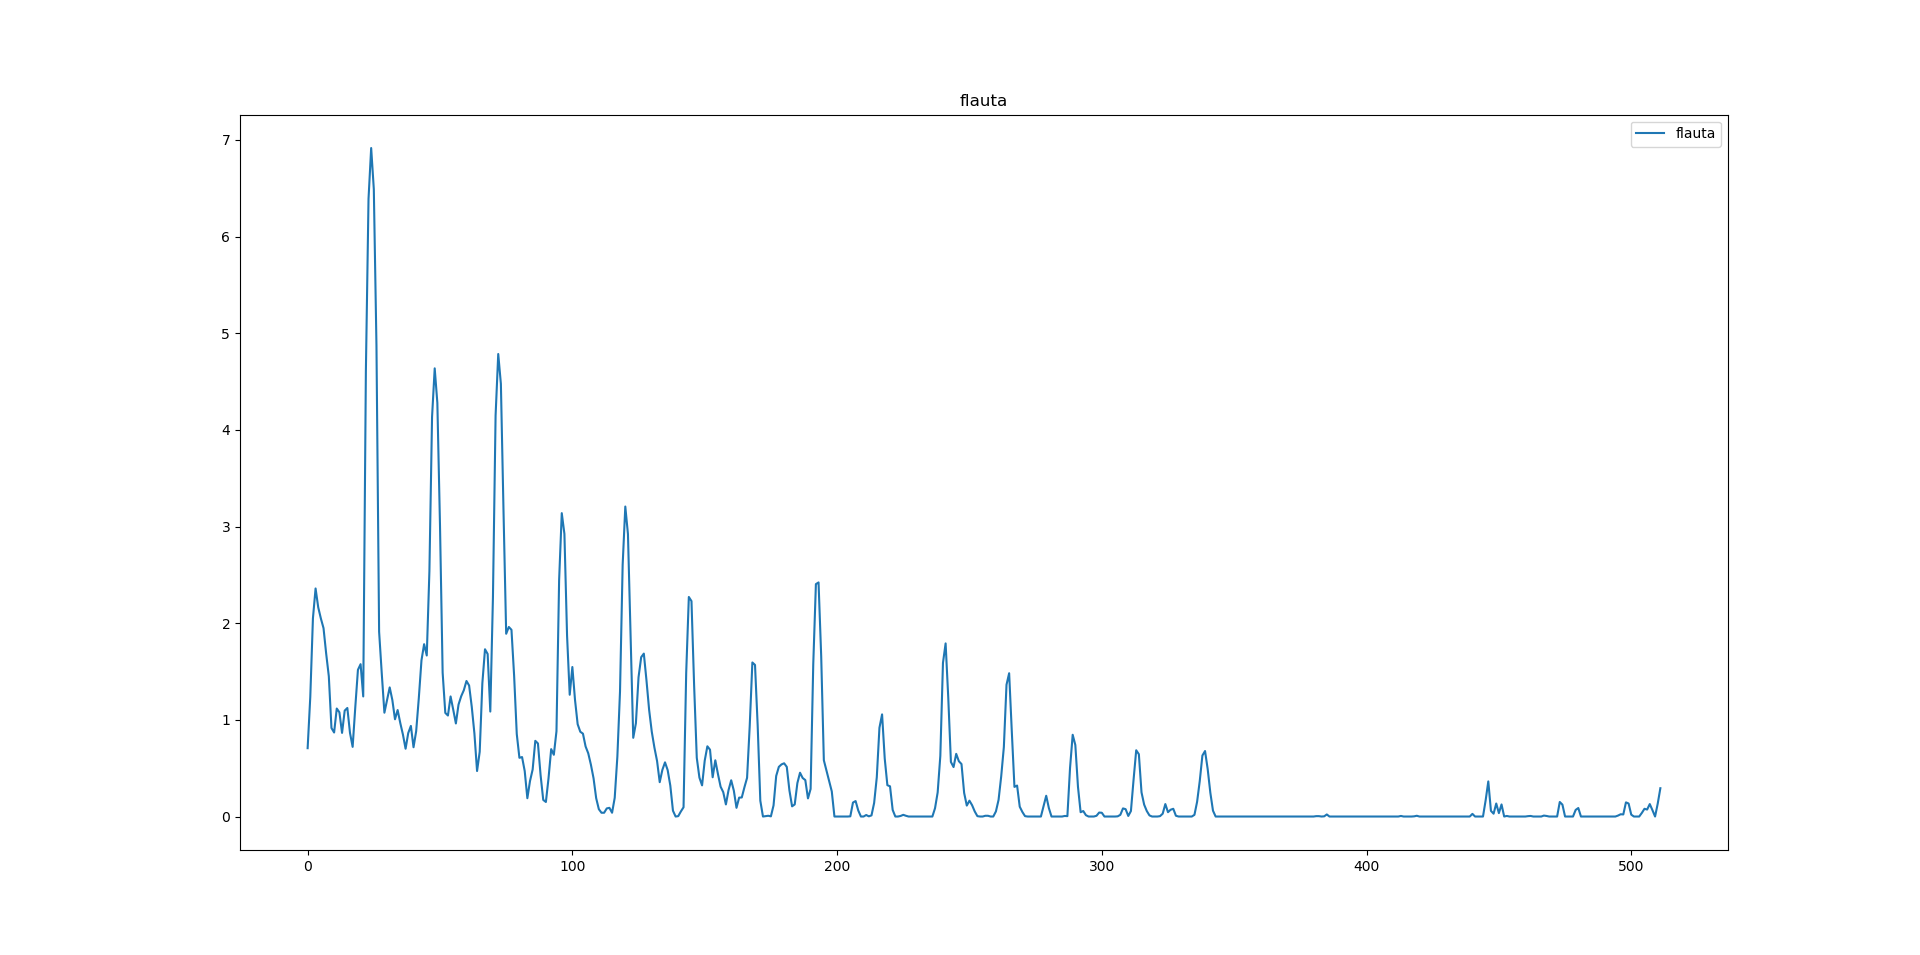
\includegraphics[width=12cm, keepaspectratio]{img/flauta512.png}
	\caption{Valores de la FFT de una flauta con 512 muestras.}\label{fig:flauta}
\end{figure}

En la figura~\ref{fig:flauta} se puede observar de una manera muy clara los distintos armónicos que podemos diferenciar en un sonido musical. Los picos son bastante claros, y finalmente acaba tendiendo a cero, pero unas muestras más tarde de lo que lo hace la figura~\ref{fig:silbido} y antes de lo que lo hará la figura~\ref{fig:yo}.


\section{Duración de los audios}
\label{sec:duracion-audio}

Para comprobar cuál podría ser la duración más propicia de los audios, se hicieron varias pruebas cambiando la duración de los audios cuando se recogen las muestras. Los valores que se colocarán son los siguientes: 250ms, 500ms y 1000ms. Para esta prueba se grabó a tres personas recitando un mismo texto.

Cuando el tiempo es de 250ms podemos observar que los picos se crean en valores más altos.

\begin{figure}
	\centering
	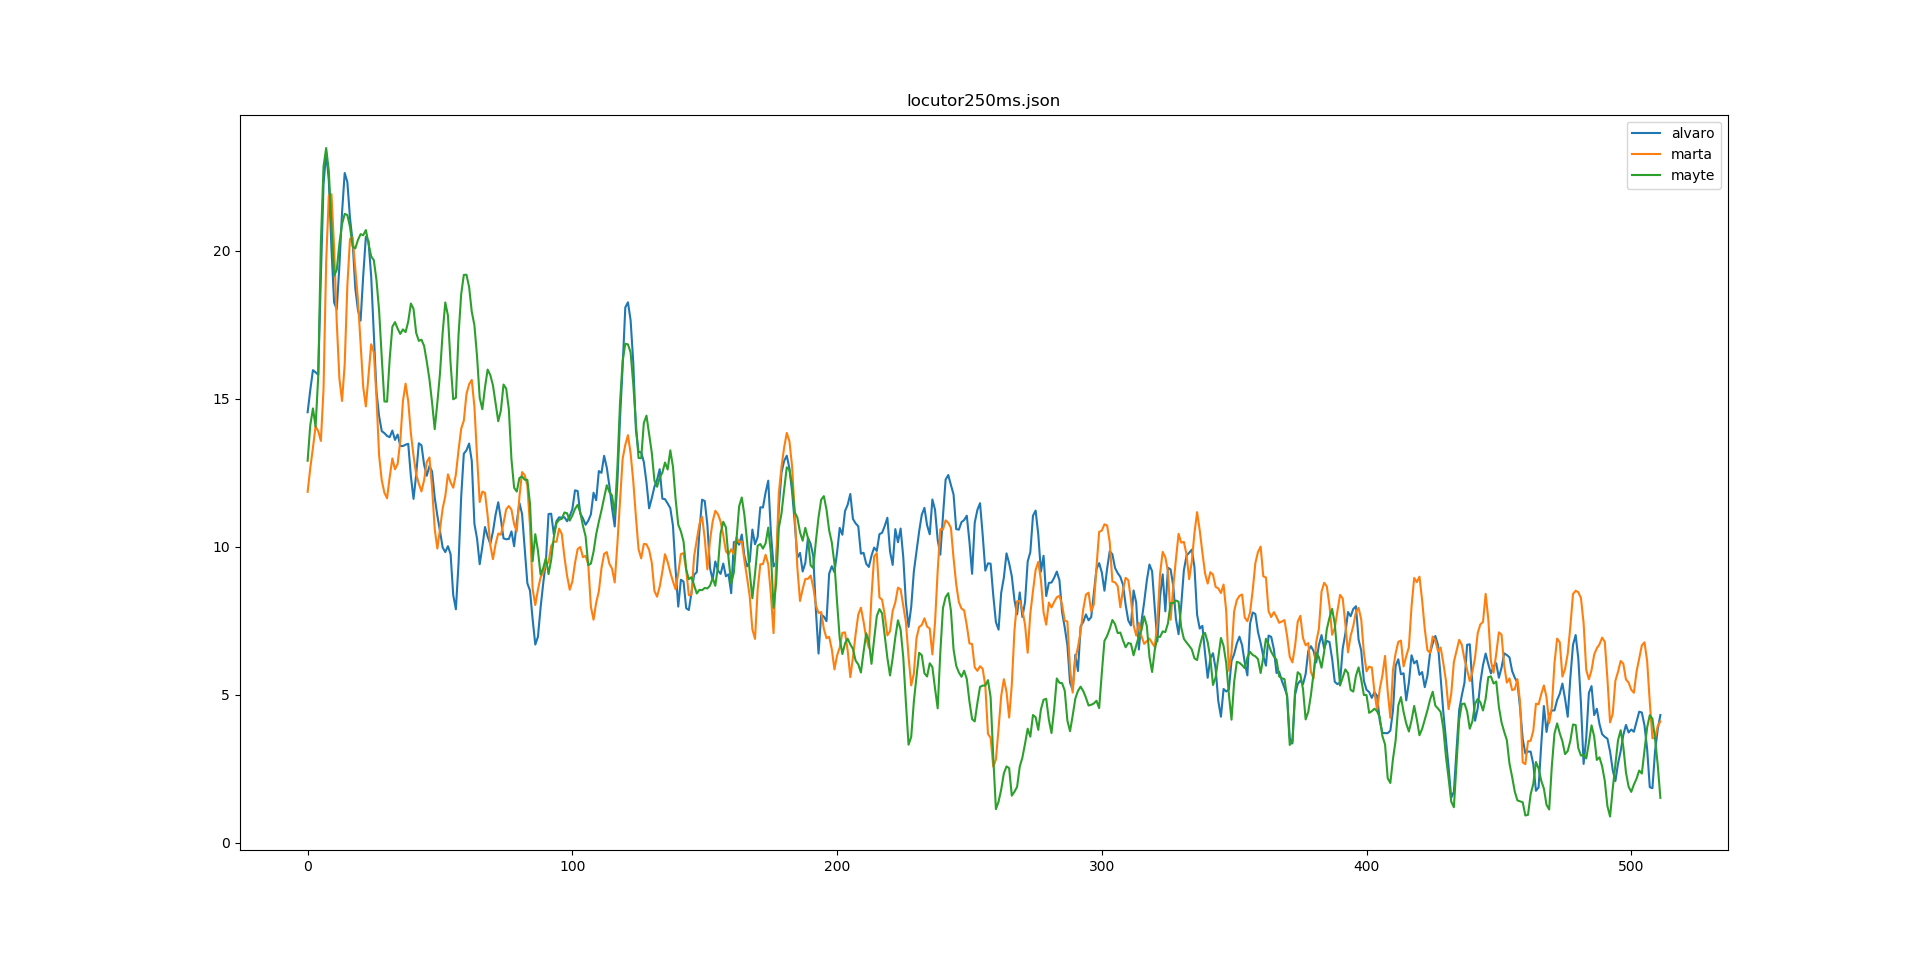
\includegraphics[width=12cm, keepaspectratio]{img/locutor250ms.png}
	\caption{Valores de la FFT con duración de 250ms.}\label{fig:locutor250ms}
\end{figure}

Cuando el tiempo es de 500ms vemos que las caídas que en la grabación de 250ms subían rápido, se mantienen en la zona baja durante más muestras.

\begin{figure}
	\centering
	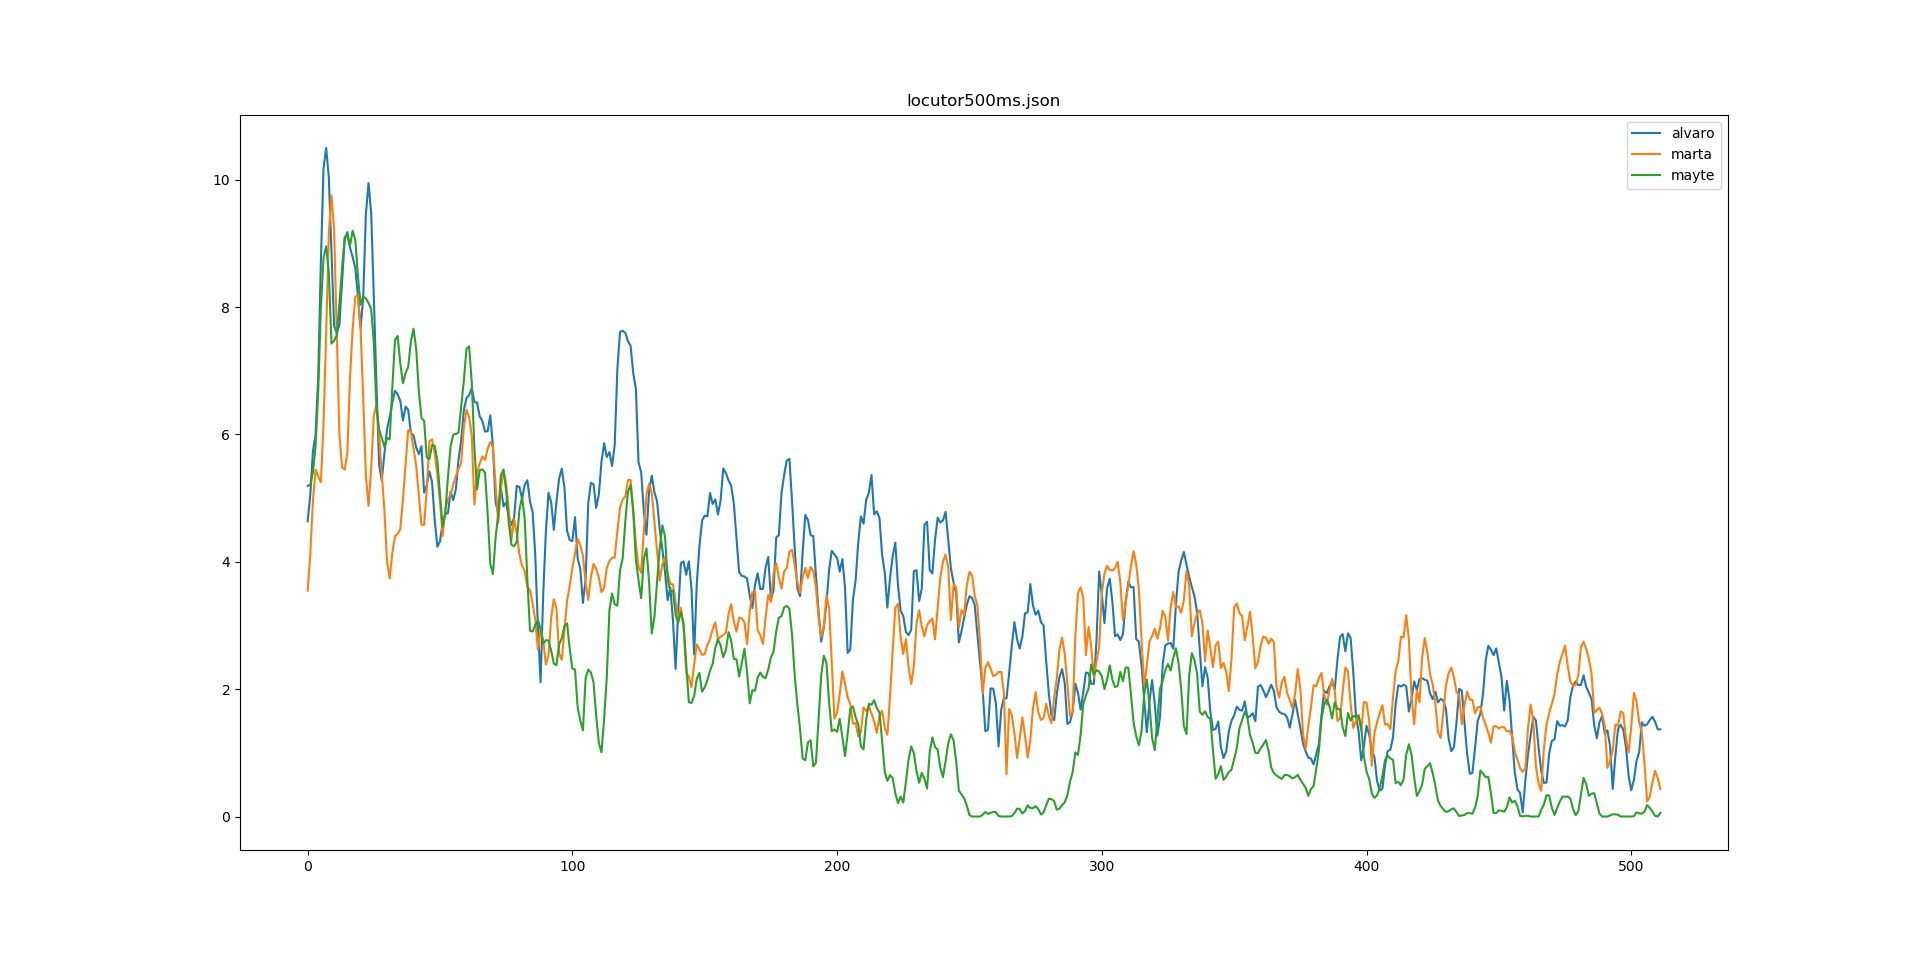
\includegraphics[width=12cm, keepaspectratio]{img/locutor500ms.png}
	\caption{Valores de la FFT con duración de 500ms.}\label{fig:locutor500ms}
\end{figure}

Cuando el tiempo es de 1000ms los picos no son tan exagerados y queda más repartido a lo largo de la gráfica.

\begin{figure}
	\centering
	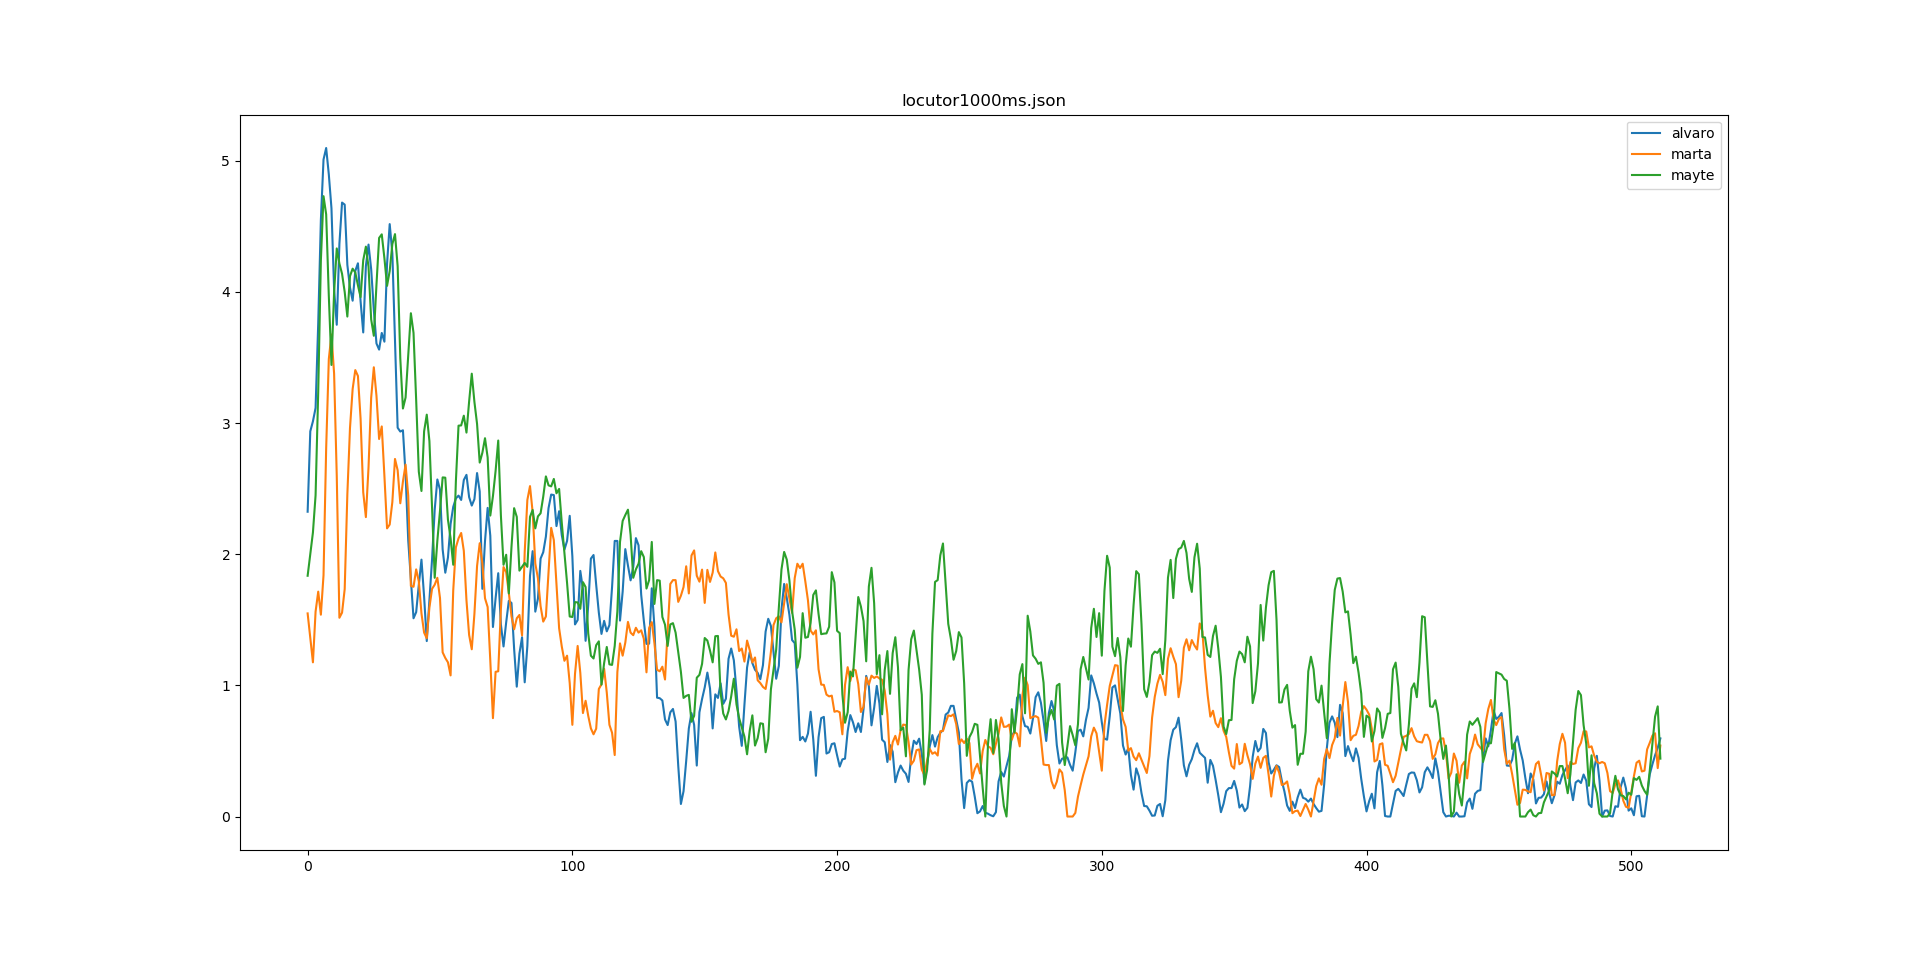
\includegraphics[width=12cm, keepaspectratio]{img/locutor1000ms.png}
	\caption{Valores de la FFT con duración de 1000ms.}\label{fig:locutor1000ms}
\end{figure}

No creo que haya una elección de tiempo que sea mejor que otra, todo depende de qué se quiera grabar. Por ejemplo, si vamos a grabar una nota obtenida de un instrumento de aire, será más conveniente colocar un tiempo bajo, para poder obtener más muestras en menos tiempo. Pero si por el contrario vamos a grabar a una persona recitando un poema, quizá sería más conveniente ponerle un tiempo más alto, porque si se cogen muchas muestras, la aplicación tarda mucho tiempo en ejecutarse.


%%%%%%%%%%%%%%%%%%%%%%%%%%%%%%%%%%%%%%%%%%%%%%%%%%%%%%%%%%%%%%%%%%%%%%%%%%%%%%%%
%%%%%%%%%%%%%%%%%%%%%%%%%%%%%%%%%%%%%%%%%%%%%%%%%%%%%%%%%%%%%%%%%%%%%%%%%%%%%%%%
% RESULTADOS %
%%%%%%%%%%%%%%%%%%%%%%%%%%%%%%%%%%%%%%%%%%%%%%%%%%%%%%%%%%%%%%%%%%%%%%%%%%%%%%%%

\cleardoublepage
\chapter{Resultados}
\label{chap:resultados}

\section{Notas musicales}
\label{sec:notas-musicales-res}

Para comprobar si los resultados que se obtenían eran correctos, se probó la realización de un modelo que reconociese notas musicales tocadas con una flauta dulce. Se crearon para este modelo siete etiquetas, cada una correspondiente a una de las notas que tenemos en una escala en clave de sol, como se muestra en la figura~\ref{fig:pentagrama}.


\begin{figure}
	\centering
	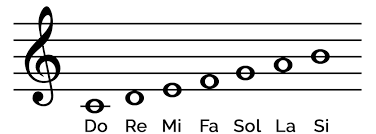
\includegraphics[width=12cm,keepaspectratio]{img/pentagrama.png}
	\caption{Pentagrama en clave de sol.}\label{fig:pentagrama}
\end{figure}

La duración escogida para las muestras de audio fue de 500ms, para que se tomaran suficientes muestras en no mucho tiempo.

\begin{figure}
	\centering
	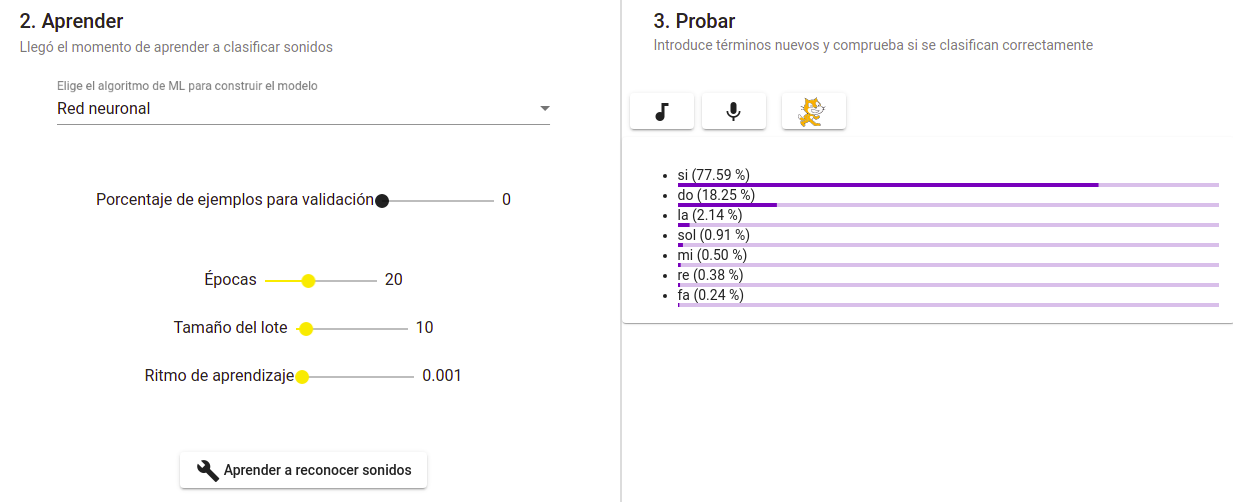
\includegraphics[width=14cm]{img/nn1.png}
	\caption{Reconocimiento de nota con Redes Neuronales.}\label{fig:neural-networks}
\end{figure}

\begin{figure}
	\centering
	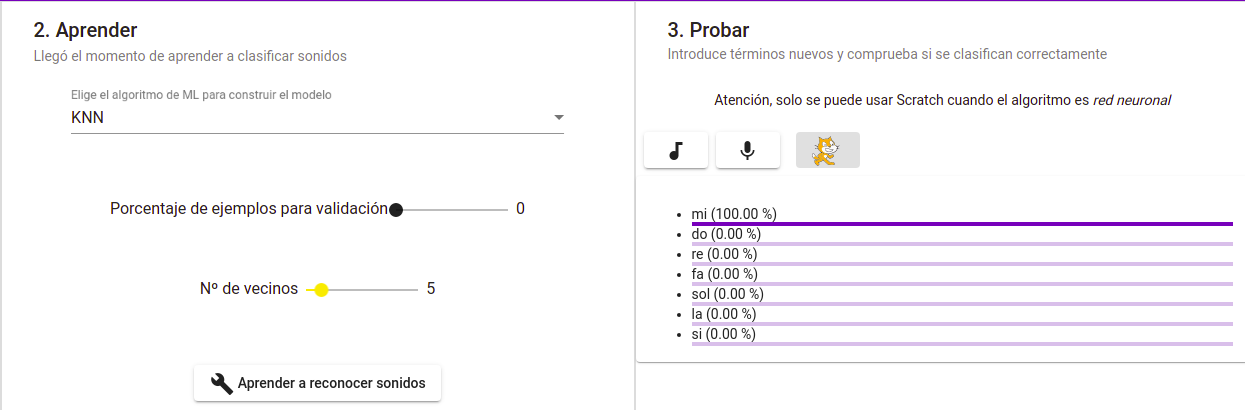
\includegraphics[width=14cm]{img/knn1.png}
	\caption{Reconocimiento de nota con KNN.}\label{fig:knn}
\end{figure}

Los resultados obtenidos fueron bastante buenos, incluso excelentes, usando redes neuronales el acierto era alto, pero aún se identificaba en porcentajes bajos como otra nota, véase la figura~\ref{fig:neural-networks}. Sin embargo al cambiar el algoritmo y utilizar KNN, los resultados son correctos, como se puede observar en la figura~\ref{fig:knn}.

Para comprender por qué se reconoce mejor mediante el uso del algoritmo de KNN que de Redes Neuronales, hay que hacer hincapié en cómo hacen la predicción cada uno delos algoritmos:

\section*{Redes Neuronales}
\label{sec:neural-networks}

El algoritmo de redes neuronales (\textit{neural networks})~\cite{izaurieta2000redes} trata de emular las conexiones que se realizan en el cerebro a la hora de tomar decisiones. Se trata de un algoritmo complicado, pero muy efectivo.

Cada uno de los nodos de la figura~\ref{fig:neural-networks-diagram} representa una neurona, y diferenciadas por colores tenemos las neuronas pertenecientes a cada una de las capas que conforman el algoritmo.

La primera capa, se encarga de analizar las características de los datos de entrada y repartirlos en función del resultado obtenido al pasarse por una función asignada a cada una de las neuronas. Este resultado se conoce como peso sináptico, y se usa para definir la importancia relativa de cada una de las entradas.

En la segunda capa, o capa oculta, el algoritmo continúa asignando pesos a cada una de las características, las capas ocultas pueden variar de tamaño, desde una o dos capas de neuronas, hasta cientos o miles de capas. Del tamaño de esta capa dependerá el tiempo que tarde en clasificarse el dato.

La última capa, o capa de salida, es la que se encarga de devolver el dato ya clasificado dentro de una etiqueta

\begin{figure}
	\centering
	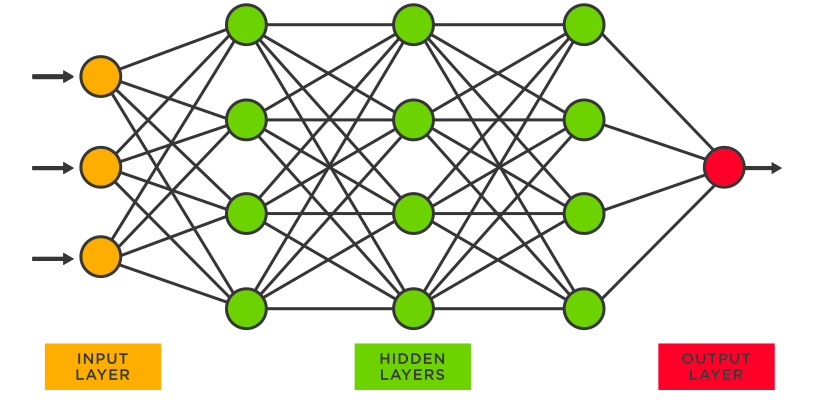
\includegraphics[width=9cm]{img/neutral-network-diagram.png}
	\caption{Diagrama del algoritmo Redes Neuronales.}\label{fig:neural-networks-diagram}
\end{figure}

\section*{KNN}
\label{sec:knn}

El algoritmo de k vecinos más cercanos (\textit{k-nearest neighbors}), conocido como \texttt{KNN}~\cite{tikariha2018comparative} es un modelo estadístico de reconocimiento supervisado de patrones.

Al comenzar, el algoritmo coloca los datos de entrenamiento en una dimensión de tamaño igual al número de características de cada dato. Después coloca el dato a clasificar en la misma dimesión, y escoge los k puntos más cercanos, teniendo en cuenta la etiqueta de cada uno de esos puntos, identifica el dato como perteneciente a esa clase. Para evitar empates entre etiquetas, los valores de k suelen ser bajos e impares.

La figura~\ref{fig:knn-diagram} expone un ejemplo de clasificación de un dato con dos características. Escogiendo una k con valor de 3, el algoritmo clasficaría el dato como perteneciente a la clase B, pero si cambiamos el valor de k de 3 a 7, el dato quedaría clasificado como clase A.

\begin{figure}
	\centering
	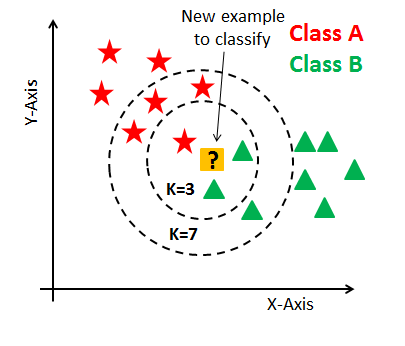
\includegraphics[width=9cm]{img/knn-diagram.png}
	\caption{Diagrama del algoritmo KNN.}\label{fig:knn-diagram}
\end{figure}

\pagebreak

Conociendo cómo funcionan ambos algoritmos y sabiendo que tenemos un total de 512 características, que es la longitud del vector de datos que se introduce, ¿por qué KNN predice de una manera más acertada que el algoritmo de redes neuronales?

En las figuras~\ref{fig:do} y~\ref{fig:si} podemos observar respectivamente las notas \textit{do} y \textit{si}, la más grave y la más aguda dentro de la escala escogida.

\begin{figure}
	\centering
	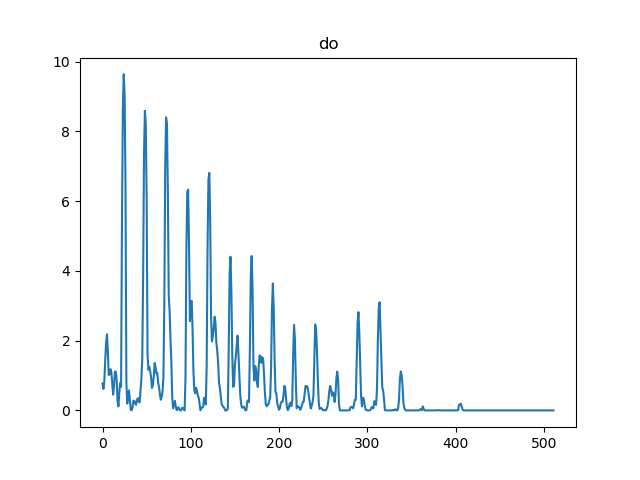
\includegraphics[width=12cm]{img/do.png}
	\caption{FFT de la nota do.}\label{fig:do}
\end{figure}

\begin{figure}
	\centering
	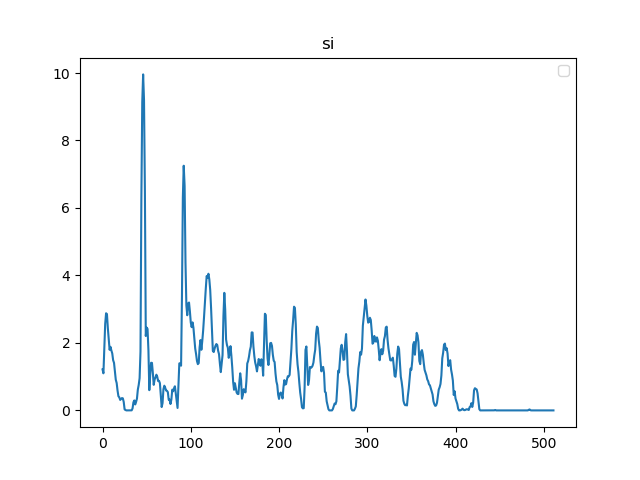
\includegraphics[width=12cm]{img/si.png}
	\caption{FFT de la nota si.}\label{fig:si}
\end{figure}

Observando los distintos armónicos dentro de cada una de las gráficas y sabiendo que cada una de las muestras es una característica a analizar, con KNN la diferenciación entre estas dos notas se podría ver de una manera sencilla.

Los picos que podemos observar en la figura~\ref{fig:do} son mucho más numerosos y están más estilizados que los que podemos observar en la figura~\ref{fig:si}, que forman picos pero con una caída mucho menor que las de la otra nota.

Por tanto, KNN sería el algoritmo más adecuado para diferenciar estas notas musicales, gracias a la forma que tienen ambas.

\section{Prueba con alumnos de instituto.}
\label{sec:prueba}

Para una última comprobación, se probó a dar la herramienta a tres alumnas de 2º de la ESO, de 13 años, y dejar que probaran su funcionalidad.

Antes de dejar que probaran la aplicación, se les plantearon dos preguntas:

\begin{itemize}
	\item ¿Qué es la \texttt{Inteligencia Artificial}?~ Ninguna de las tres alumnas escogidas supo responder correctamente la pregunta. No obstante, elaboraron una definición algo cercana a lo que se podía esperar: ``Es la capacidad de un ordenador de hacer cosas que podríamos hacer nosotras'', dijeron al final.
	\item ¿Qué es el \texttt{Machine Learning}?~ De nuevo, no supieron definir bien qué podía ser el \texttt{Machine Learning}. Aun así, consiguieron elaborar una respuesta, simplemente traduciendo de manera literal: ``Aprender máquina, o sea hacer que un ordenador aprenda cosas nuevas'' fue su respuesta final.
\end{itemize}

Después de una breve explicación sobre el funcionamiento de la aplicación usando algunos de los ejemplos de prueba que se han descrito antes, ver sección~\ref{sec:notas-musicales-res} y capítulo~\ref{chap:experimentos-validacion} y creando un ejemplo nuevo en el momento para el reconocimiento de vocales, ver figuras~\ref{fig:reconocimiento-vocales-nn} y~\ref{fig:reconocimiento-vocales-knn}, así como una breve teoría del funcionamiento de las redes neuronales y KNN, ver capítulo~\ref{sec:notas-musicales-res}, y del significado de la matriz de confusión y de la tabla de evolución de aprendizaje, ver sección~\ref{chap:experimentos-validacion} y figuras~\ref{fig:learning-evolution} y~\ref{fig:matriz-confusion}, se les dio vía libre para que ``jugaran'' con la herramienta. Es cierto que al principio no fueron capaces de verle la utilidad, pero según iba pasando el tiempo, cada vez hacían experimentos más interesantes.

\begin{figure}
	\centering
	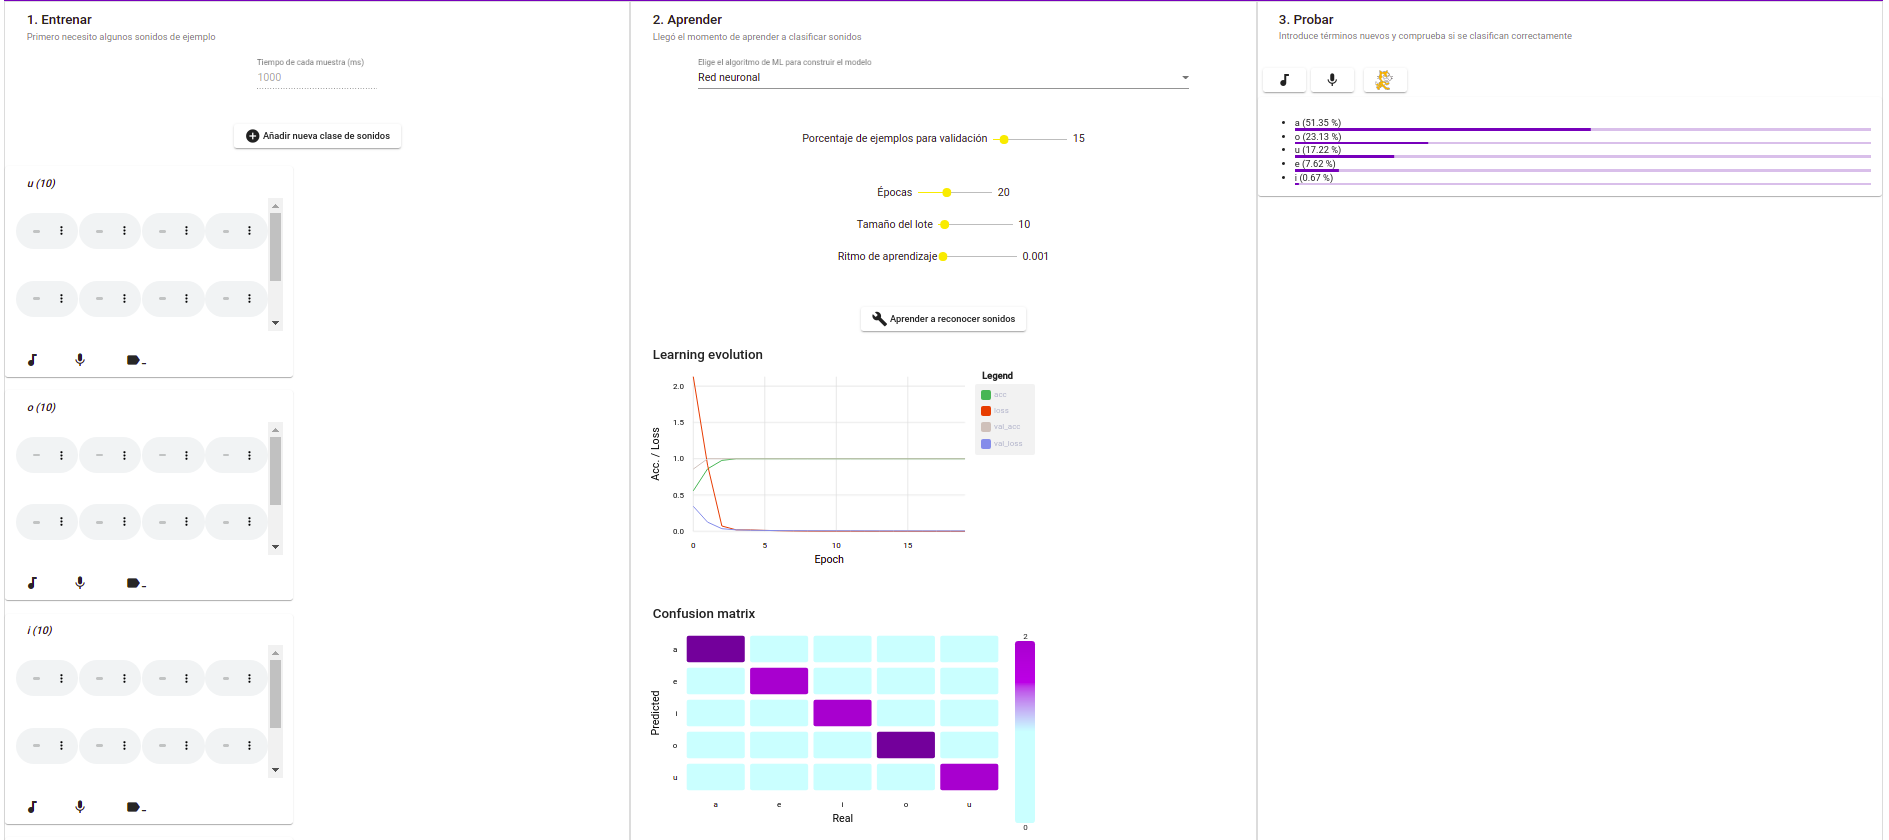
\includegraphics[width=14cm]{img/vocales-nn.png}
	\caption{Reconocimiento de vocales con redes neuronales.}\label{fig:reconocimiento-vocales-nn}
\end{figure}

\begin{figure}
	\centering
	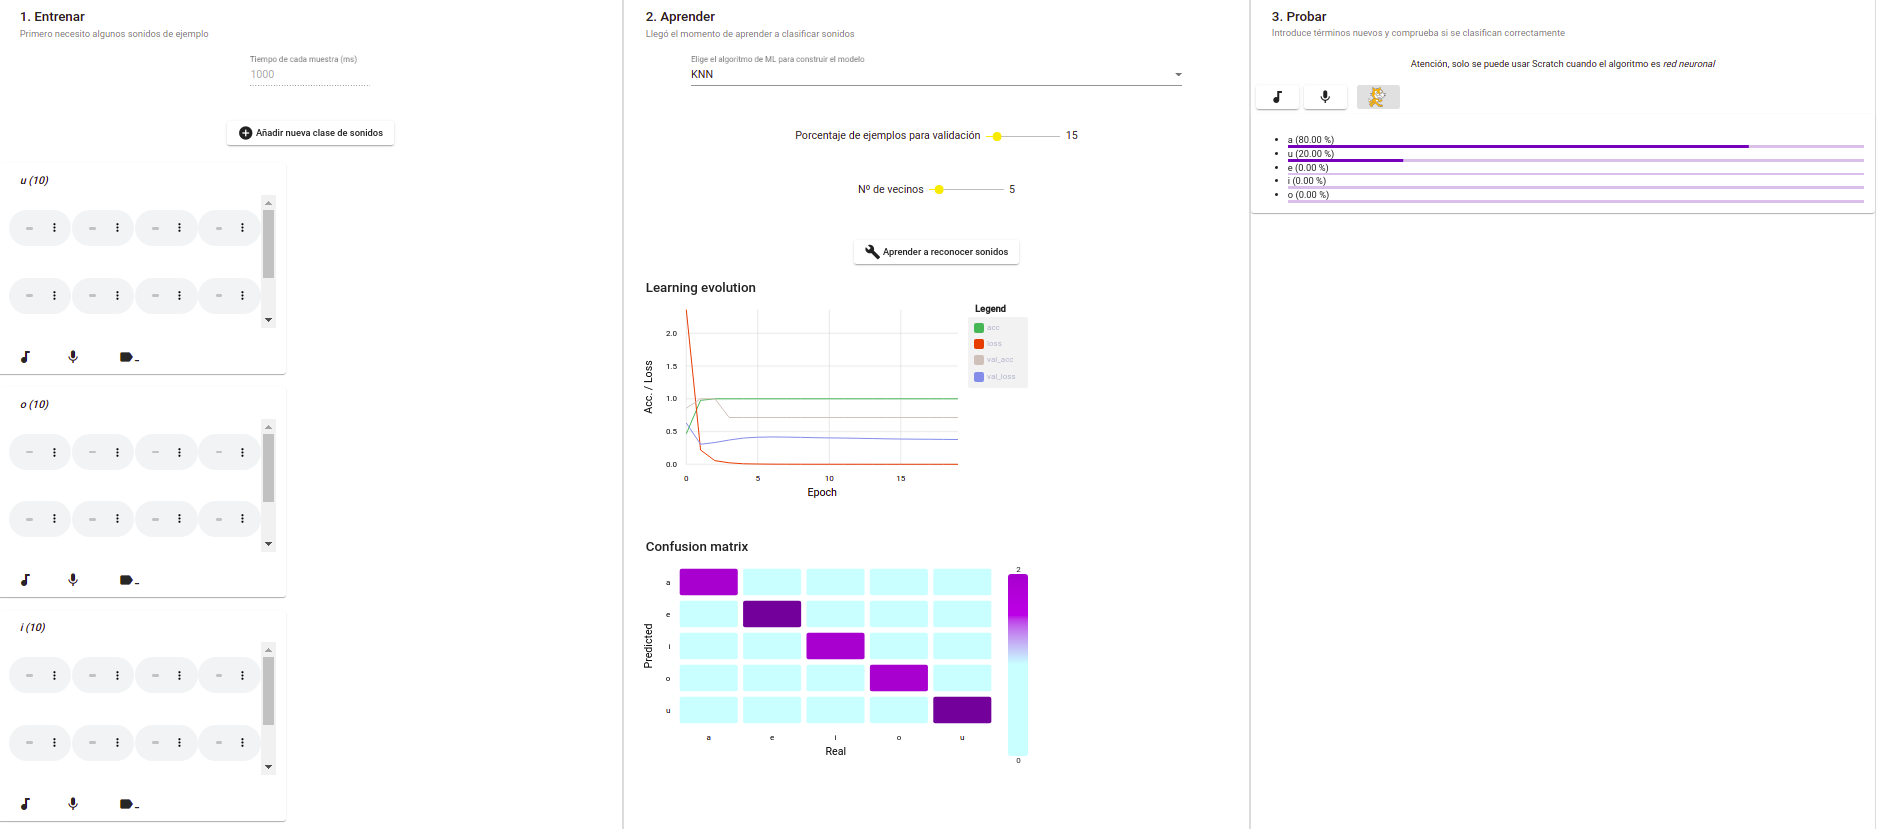
\includegraphics[width=14cm]{img/vocales-knn.png}
	\caption{Reconocimiento de vocales con KNN.}\label{fig:reconocimiento-vocales-knn}
\end{figure}

Los primeros experimentos se basaron en emular el de las notas musicales, con una flauta dulce que tenían de la asignatura de música que imparten en el instituto, pero decidieron cambiar las notas a analizar, e incluso aumentaron el tiempo de grabación para coger alguna parte de una canción que sabían tocar, pese a que el ruido de fondo era alto y no era fácil diferenciar los extractos de canción, la aplicación funcionó de una manera bastante acertada.

En el siguiente experimento plantearon la posibilidad de reconocer partes de canciones, aumentando la duración de los audios a 2000ms. Grabaron el principio de tres canciones, que se reprodujeron desde el móvil. Si bien el resultado no salía correcto al 100\%, porque únicamente se recogía una muestra muy larga, es cierto que la herramienta acertó en un porcentaje bastante aceptable.

Este último experimento les ayudó a comprender que la herramienta funciona mejor a cuantas más muestras se le facilite, en ese momento les pedí que me explicaran por qué creían que no funcionaba bien cuando tenía pocas muestras, a lo que respondieron: ``Si no se le enseña bien, no puede saberlo todo, ¿no?''. \\En este momento me decidí por explicarles los distintos tipos de aprendizaje que presenta el \texttt{Machine Learning}, ver sección~\ref{sec:machine-learning}, así como el tipo de aprendizaje con el que cuenta la aplicación.

Otro experimento que se les ocurrió fue, pensando en \texttt{Alexa}, enseñar a la herramienta a reconocer palabras. Para ponerse a ello pensaron en palabras que pudieran decir en un segundo, y poniendo el tiempo de grabación en 1000ms, iban alternándose para decir la palabra en cuestión. Escogieron tres palabras: silla, pan y mesa. Los resultados obtenidos en esta parte fueron buenos. Además de que dejó sorprendidas a las alumnas en cuestión.

Ya habiendo probado el reconocimiento de sonido, decidieron probar el reconocimiento de imágenes, que ciertamente les resultó más entretenido, en resumen: les gusta saber quién se parece más a quién.

Para probar la funcionalidad del reconocimiento de texto se les pidió que pensaran en palabras y las agrupasen, para esto pensaron en diferenciar entre singulares y plurales, una idea interesante a mi parecer, para ello colocaron varias palabras en singular y plural en dos etiquetas diferentes, después probaron con palabras distintas a las que se habían escogido, el resultado como cabía esperar fue bueno, tanto usando KNN como con redes neuronales.

Para finalizar el experimento, se les volvió a repetir las mismas preguntas. En esta ocasión las respuestas fueron más concisas y acertadas:

\begin{itemize}
	\item ¿Qué es la \texttt{Inteligencia Artificial}?~ A lo que respondieron: ``La capacidad de las máquinas de hacer cosas que sólo podríamos hacer los seres humanos'', una definición bastante acertada a mi parecer.
	\item ¿Qué es el \texttt{Machine Learning}?~ Su respuesta fue: ``Es como una parte de la \texttt{Inteligencia Artificial}, como la más importante'', mejorando con esta respuesta su definición anterior.
\end{itemize}

Además, se les planteó una última pregunta:

\begin{itemize}
	\item ¿Para qué se podría utilizar el \texttt{Machine Learning}? Sus respuestas a esta pregunta fueron fascinantes, ya que les hizo pensar y dedujeron que todos los móviles funcionan usando, de alguna manera, el \texttt{Machine Learning}, ya sea para el reconocimiento facial o el dactilar o incluso los anuncios que aparecen en las redes sociales. También propusieron ideas, como la de usar el reconocimiento facial para buscar a ``gente mala'' mediante cámaras de comercios o lugares públicos.
\end{itemize}

En conclusión, creo que fue una buena experiencia para ellas, que aprendieron algo nuevo y, sobre todo, pasaron un buen rato, aprendiendo entre risas, que al final es el objetivo que se persigue con esta aplicación.

%FIXME: detallar más por qué eso es así a partir de lo que se ve en la figura.


%%%%%%%%%%%%%%%%%%%%%%%%%%%%%%%%%%%%%%%%%%%%%%%%%%%%%%%%%%%%%%%%%%%%%%%%%%%%%%%%
%%%%%%%%%%%%%%%%%%%%%%%%%%%%%%%%%%%%%%%%%%%%%%%%%%%%%%%%%%%%%%%%%%%%%%%%%%%%%%%%
% CONCLUSIONES %
%%%%%%%%%%%%%%%%%%%%%%%%%%%%%%%%%%%%%%%%%%%%%%%%%%%%%%%%%%%%%%%%%%%%%%%%%%%%%%%%

\cleardoublepage
\chapter{Conclusiones}
\label{chap:conclusiones}

Considero que el trabajo realizado ha sido bastante bueno, ya que crear un analizador de audio que no sirva únicamente para una sola función (diferenciar vocales, diferenciar notas musicales, diferenciar locutores, entre otros) es una tarea complicada, no obstante, el resultado ha sido interesante y la funcionalidad de lo creado es bastante interesante.

\section{Consecución de objetivos}
\label{sec:consecucion-objetivos}

Al comenzar el proyecto se propusieron varios objetivos, que se han cumplido todos.

En el aspecto del análisis y reorganización de la estructura de \texttt{LearningML}, se puede decir que ahora está bien organizada y que los componentes y servicios creados siguen la línea de lo que ya estaba anteriormente.

Y en cuanto al análisis de las señales de audio, al final resultó más óptimo para la consecución del trabajo que no se buscaran aspectos específicos, sino que se guardaran todas las bandas de frecuencia obtenidas y se realizara la predicción basándose en esos aspectos.

\section{Aplicación de lo aprendido}
\label{sec:aplicacion}

En el aspecto de desarrollo web ha sido de gran ayuda tener conocimientos básicos, que pude adquirir en \textit{Construcción de Servicios y Sistemas Audiovisuales en la Web}, además para el desarrollo de aplicaciones web, pese a que no fue en Angular, sino en Django y Node.js, la asignatura de \textit{Laboratorios de Tecnologías Audiovisuales en la Web} fue de gran ayuda, ya que no se comienza de cero en el tema del uso de plantillas y lenguaje de plantillas.

También ha sido de gran utilidad el saber cómo llevar a cabo un programa de manera eficiente y limpia, esto se lo debo a \textit{Informática II}, que gracias a un lenguaje tan altamente tipado y complicado como Ada hizo que el orden tomara una posición importante a la hora de realizar cualquier programa o aplicación.

Además las asignaturas de \textit{Tratamiento Digital del Sonido} y \textit{Tratamiento Digital de la Imagen} fueron de gran ayuda a la hora tanto de comprender cómo funcionaban los distintos algoritmos, como de realizar el análisis de audio, pese a que al final no se buscó ninguna de las características que podrían diferenciar un audio de otro.


\section{Lecciones aprendidas}
\label{sec:lecciones_aprendidas}

%FIXME: desarrolla estos puntos, que no quede como una lista.
\section*{Desarrollo de aplicaciones con Angular.}

Angular es un \texttt{framework} que me ha parecido de lo más útil, al menos para el desarrollo de aplicaciones web. La construcción de la aplicación se hace de una manera muy sencilla, gracias al comando \texttt{ng new [nombre-app]}, que permite crear el esqueleto completo de la aplicación, ahorrando mucho tiempo al comienzo. De igual manera, la creación de componentes, servicios y demás, hacen de Angular una herramienta muy útil.

\section*{Análisis de audio con la API web.}

Pese a que en el inicio fue complicado conseguir introducirlo dentro de la aplicación, la API web de audio proporciona unas herramientas que pueden resultar muy útiles, ya no solo a la hora de realizar tareas como esta, sino para editar \textit{streams} de audio.

El uso de la interfaz de \texttt{AudioContext} en principio pudo suponer un problema, pero una vez se comprende el funcionamiento y las posibilidades que ofrece, ves que el tratamiento de audio en la web se vuelve relativamente sencillo.

\section*{Programación asíncrona.}

Al comenzar el proyecto conocía lo que era la programación asíncrona, pero no sabía de qué forma implementarla, ni las facilidades que ésta podía acarrear.

Después de investigar y hacer multitud de pruebas, creo que puedo decir con certeza que es una de las cosas que más me alegro de haber aprendido, por la cantidad de posibilidades que abre dentro del desarrollo de una aplicación que funciona en tiempo real.

\section*{TypeScript.}

Al estar basado en \texttt{JavaScript} no me resultó excesivamente complicado de comprender la sintaxis que ofrecía, pese a que tiene algunos cambios respecto de su lenguaje padre, son cambios que son sencillos e intuitivos.

Por tanto, \texttt{TypeScript} me parece un lenguaje muy útil, ya que toma todas las cosas buenas de \texttt{JavaScript} y fortalece los puntos débiles que tuviera este lenguaje.

\section{Trabajos futuros}
\label{sec:trabajos_futuros}

Una de las principales carencias del análisis de audio en \texttt{LearningML} es la forma de recoger muestras de sonidos, quizá una cambio en la interfaz en ese aspecto pudiera solucionarlo. Además a la hora de realizar las pruebas, sería muy interesante no tener que parar de grabar para analizar, sino que continúe grabando una vez haya analizado y mostrando la resolución, hasta que el usuario decida parar la grabación, cambiando cada vez que se grabe una muestra el valor predicho.

En un aspecto similar al análisis de audio, el análisis de imágenes podría llevar un crecimiento paralelo al de audio.

El \texttt{Machine Learning} no tiene límites, se puede usar para el reconocimiento de multitud de cosas, por ejemplo, una funcionalidad que permita encontrar patrones dentro de un número enorme de datos podría ser de bastante utilidad.

%%%%%%%%%%%%%%%%%%%%%%%%%%%%%%%%%%%%%%%%%%%%%%%%%%%%%%%%%%%%%%%%%%%%%%%%%%%%%%%%
%%%%%%%%%%%%%%%%%%%%%%%%%%%%%%%%%%%%%%%%%%%%%%%%%%%%%%%%%%%%%%%%%%%%%%%%%%%%%%%%
% BIBLIOGRAFIA %
%%%%%%%%%%%%%%%%%%%%%%%%%%%%%%%%%%%%%%%%%%%%%%%%%%%%%%%%%%%%%%%%%%%%%%%%%%%%%%%%

\cleardoublepage

% Las siguientes dos instrucciones es todo lo que necesitas
% para incluir las citas en la memoria
\bibliographystyle{abbrv}
\bibliography{memoria}  % memoria.bib es el nombre del fichero que contiene
% las referencias bibliográficas. Abre ese fichero y mira el formato que tiene,
% que se conoce como BibTeX. Hay muchos sitios que exportan referencias en
% formato BibTeX. Prueba a buscar en http://scholar.google.com por referencias
% y verás que lo puedes hacer de manera sencilla.
% Más información: 
% http://texblog.org/2014/04/22/using-google-scholar-to-download-bibtex-citations/

\end{document}
